% kuleuventheme2 by Janez Kren, September 2017, janez.kren@kuleuven.be, based on:
% kuleuventheme 1.3 by Roland Pastorino, 2013 roland.pastorino@kuleuven.be / www.rolandpastorino.com

\documentclass[11pt,t]{beamer}
\usetheme{kuleuven2}	%THEME OPTIONS for LOGO: kul (default), kulak, lrd,    ; OPTIONS for TITLE PAGE: normal (default), sedes


%%% OTHER SETTINGS
\usefonttheme[onlymath]{serif}			% math font with serifs, delete to make it sans-serif
\setbeamertemplate{footline}[body] 		% delete this line to remove footline bar on all frames
\usepackage[orientation=landscape,size=custom,width=16,height=9,scale=0.5,debug]{beamerposter} %enable for widescreen 16:9 ratio
%\titlegraphic{ \includegraphics[width=.2\paperwidth]{mytitlepagepic.png} } %optional title page image


%%% ADDED PACKAGES:
\usepackage[english]{babel}
\usepackage{amsfonts}
\usepackage{amssymb}
\usepackage{graphicx}

\graphicspath{{images/}} 

\newcommand{\Int}{\int\limits}


%%% TITLE PAGE INFO:
\title[The Role of Bioreactors in Tissue Engineering]{The Role of Bioreactors in Tissue Engineering} %[] will appear in footline
\subtitle{And Using Jupyter Notebooks to Teach the Fundamental Concepts of Bioreactors and Mass Transfer More Effectively}

\author{Mojtaba Barzegari}
\institute{Biomechanics Section, Department of Mechanical Engineering}
\date{November 2018}




\begin{document}
\csname beamer@calculateheadfoot\endcsname %recalculate head and foot dimension

% Title page
\begin{frame}[plain,noframenumbering]
	\titlepage
\end{frame}
	

% Table of Contents
\begin{frame}{Outline}
			\setstretch{0.6}
	\hfill	{\large \parbox{.961\textwidth}{\tableofcontents[hideothersubsections]}}
\end{frame}

\section{Introduction}
\begin{frame}[fragile]{Tissue Engineering}  
	\begin{columns}[t]
		\begin{column}{.5\textwidth}
			Tissue Engineering (TE) focuses on developing ideal tissue replacements that adequately mimic, or are functionally equivalent to, native tissues.
		\end{column}
		\begin{column}{.5\textwidth}
			\vspace{-30pt}
			\begin{figure}
			\centering
			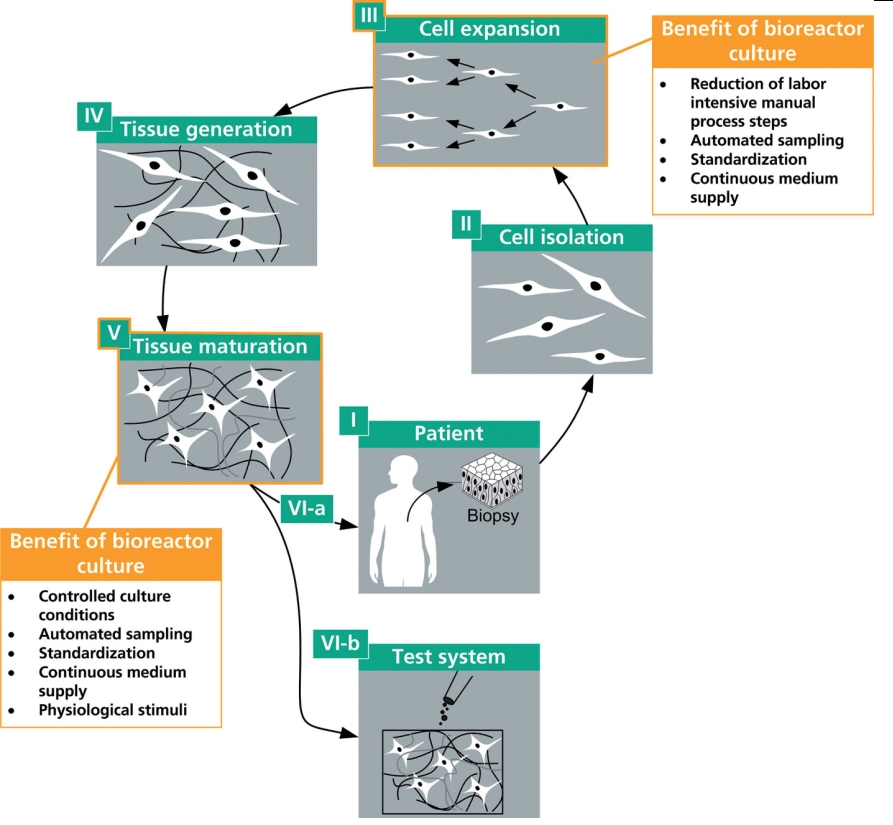
\includegraphics[width=0.9\textwidth]{te_paradigm1}
			\end{figure}
		\end{column}
	\end{columns}	
	
	\footnotesize(Jan Hansmann et al., 2013)

\end{frame}
 
\begin{frame}[fragile]{Tissue Engineering}  

	\begin{columns}[t]
		\begin{column}{.55\textwidth}
			TE aims to develop methods and technologies to create tissue constructs \emph{in vitro} that have tissue-specific \textbf{morphological}, \textbf{biological}, \textbf{chemical}, and \textbf{mechanical} properties, as well as \textbf{functions} similar to those found \emph{in vivo}.
		\end{column}
		\begin{column}{.45\textwidth}
			\vspace{-30pt}
			\begin{figure}
			\centering
			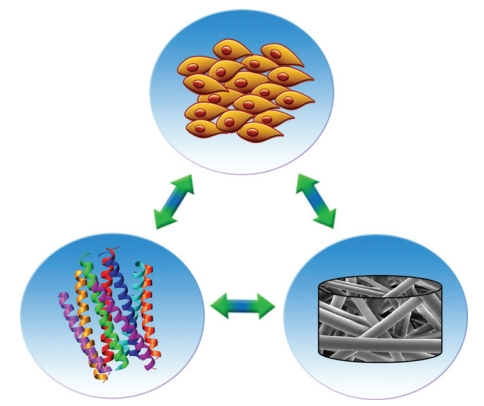
\includegraphics[width=0.9\textwidth]{te_paradigm2}
			
			\footnotesize	TE Paradigm: Cells, Scaffolds, and Signals
			\end{figure}
		\end{column}
	\end{columns}	
	
	\footnotesize(E. J. Levorson, 2011)

\end{frame}

\begin{frame}[fragile]{TE Fundamental Challenges}  

Major obstacles to the generation of functional tissues:

\begin{itemize}
\item
Limited understanding of physicochemical culture parameters
\item
High manufacturing costs
\end{itemize}

Solutions:

\begin{itemize}
\item
Enabling reproducible and controlled changes of environmental factors
\begin{itemize}
\item
Technological
means to reveal fundamental mechanisms
\item
Improve
the quality of engineered tissues
\end{itemize}
\item
Automating and standardizing tissue manufacture in
controlled systems
\end{itemize}


\footnotesize(I. Martin et al., 2004)

\end{frame}


\section{Bioreactors and Scaffolds}
\begin{frame}[fragile]{Bioreactors}  

Generally defined as devices in which
biological and/or biochemical processes develop under
closely monitored and tightly controlled environmental
and operating conditions, such as:
\begin{itemize}
\item
pH
\item
Temperature
\item
Pressure
\item
Nutrient supply
\item
Waste removal
\end{itemize}
\end{frame}


\begin{frame}[fragile]{Role of Bioreactors}  

\emph{Ex vivo} engineering of 3D tissues:

	\begin{columns}[t]
		\begin{column}{.45\textwidth}
\begin{itemize}
\item
Cell seeding
\item
Nutrition supply
\item
Stimulation as a guide
\end{itemize}
		\end{column}
		\begin{column}{.55\textwidth}
			\vspace{-10pt}
			\begin{figure}
			\centering
			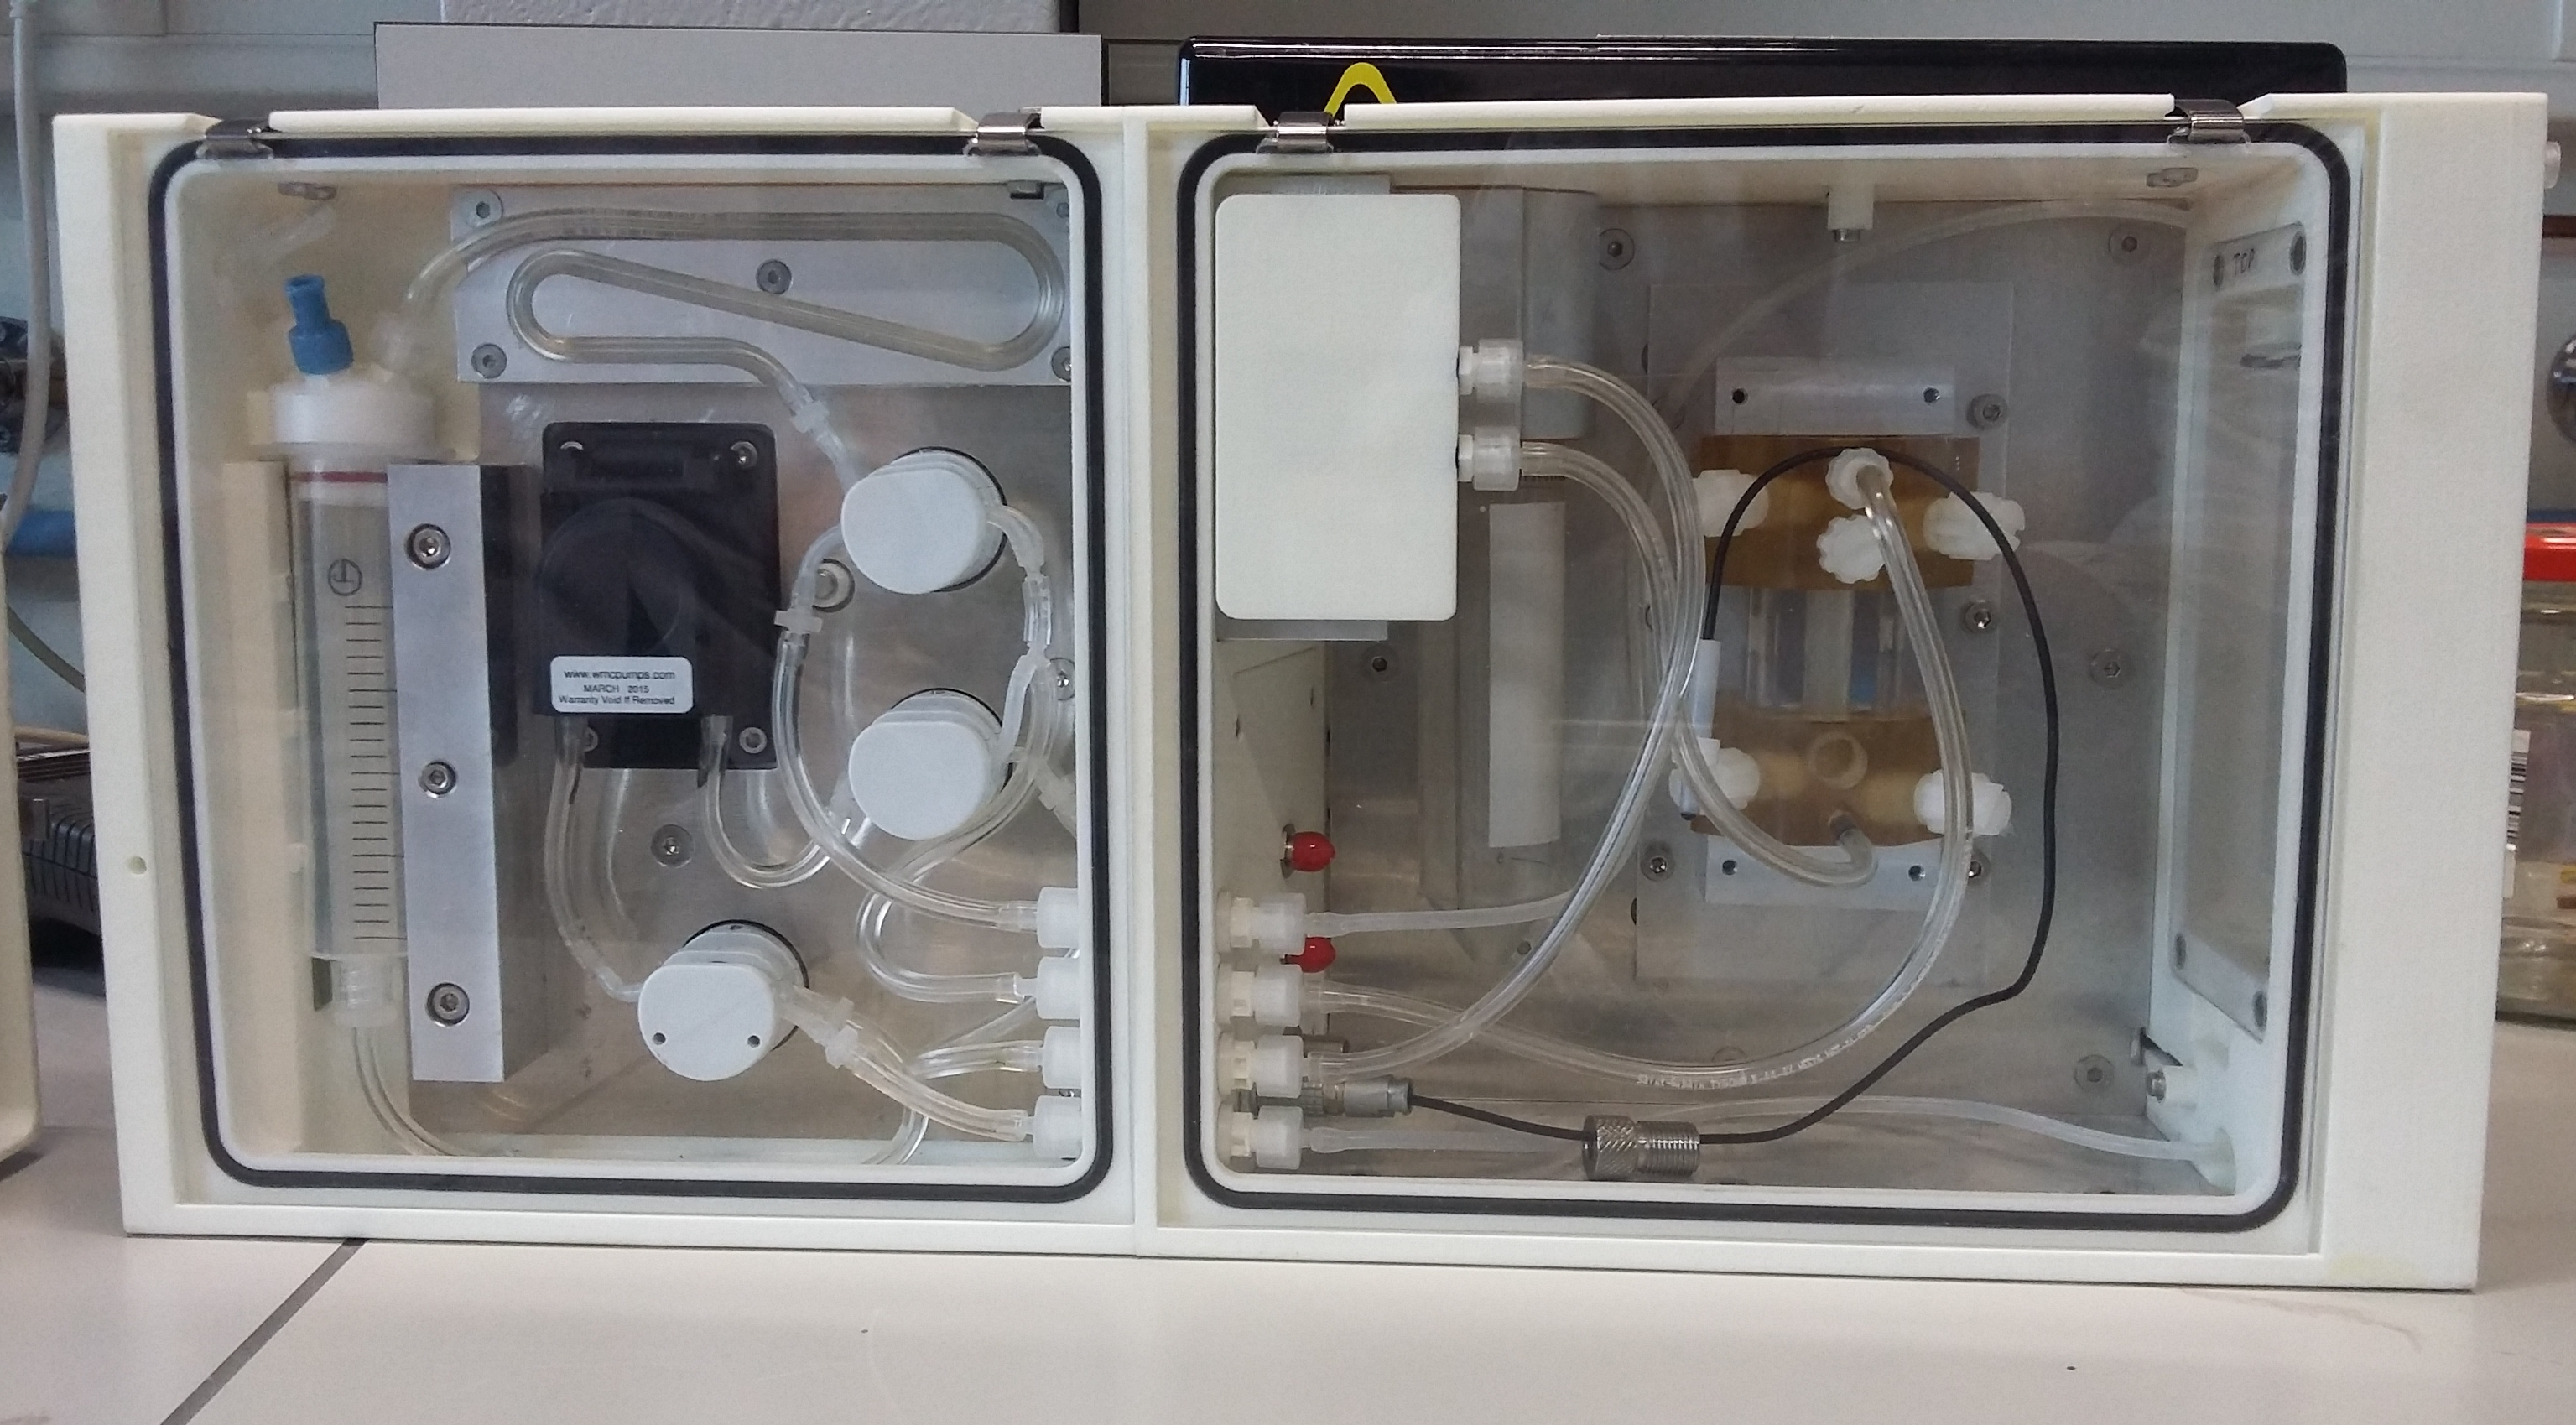
\includegraphics[width=0.9\textwidth]{prometheus}
			
			\footnotesize	Prometheus Perfusion Bioreactor
			\end{figure}
		\end{column}
	\end{columns}	
	
\end{frame}


\begin{frame}[fragile]{Cell Seeding}  

Cells should be seeded with the
highest possible efficiency (\textbf{density} and \textbf{uniformity}).
\begin{itemize}
\item
Static cell seeding
\begin{itemize}
\item
Low seeding efficiencies
\item
Non-uniform distributions of cells
\item
Diffusion is the main source of transport
\end{itemize}
\item
Dynamic cell seeding
\begin{itemize}
\item
Using principle of convective transport
\item
Using direct flow perfusion
\item
Yielding more-uniformly seeded scaffolds
\end{itemize}
\end{itemize}
\end{frame}


\begin{frame}[fragile]{Nutrition Supply (Increase Mass Transfer)}  

\begin{itemize}
\item
Perfusion of medium $\rightarrow$  increasing the mass transport of nutrients and oxygen
\item
The effects of direct perfusion depends on:
\begin{itemize}
\item
Medium flow-rate
\item
The maturation stage of the constructs
\end{itemize}
\item
The optimal operation conditions of a bioreactor should
not be determined through a trial-and-error approach $\Rightarrow$ Quantitative Models
\end{itemize}

\end{frame}


\begin{frame}[fragile]{Stimulation for Guiding Tissue Structure}  

	\begin{columns}[t]
		\begin{column}{.45\textwidth}
		 In a complex environment,
a cell is exposed to 
		\begin{enumerate}[i.]
		\item
		electrical
		\item
		electromagnetic
		\item
		 biochemical
		\item
		cell-cell interactions
		\item		
		mechanical forces 
		\item
		cell-matrix interactions 
		\end{enumerate}
 
		\end{column}
		\begin{column}{.55\textwidth}
			%\vspace{-30pt}
			\begin{figure}
			\centering
			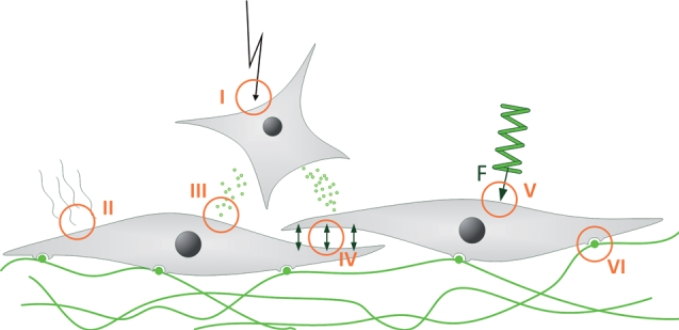
\includegraphics[width=0.9\textwidth]{stimuli}
			
			\footnotesize	Different stimuli guide cell behavior
			\end{figure}
		\end{column}
	\end{columns}	
		
	\vfill
	\footnotesize(J. Hansmann et al., 2013)

\end{frame}


\begin{frame}[fragile]{Mechanical Stimulation}  

	\begin{columns}[t]
		\begin{column}{.45\textwidth}
		 Loading conditions used in bioreactors for tissue engineering:
		\begin{enumerate}[A.]
		\item
		Uniaxial stretch
		\item
		Shear stress
		\item
		 Pressure
		\item
		Compression
		\item		
		Bending 
		\item
		Torsion 
		\end{enumerate}
 
		\end{column}
		\begin{column}{.55\textwidth}
			\vspace{-15pt}
			\begin{figure}
			\centering
			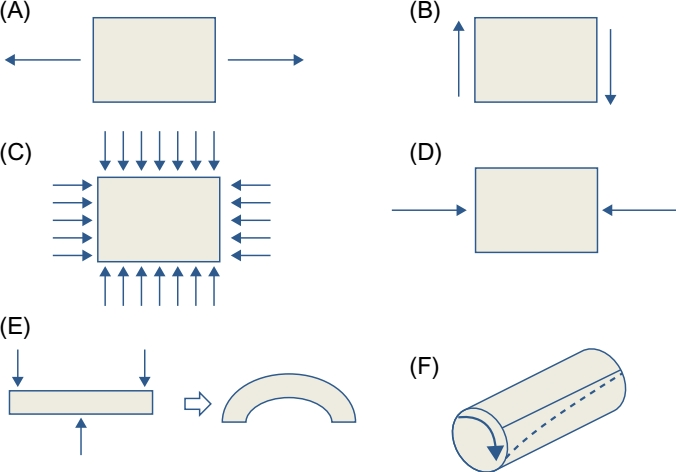
\includegraphics[width=0.9\textwidth]{loads}
			
			\end{figure}
		\end{column}
	\end{columns}	
		
	\vfill
	\footnotesize(K. J. Blosea et al., 2014)

\end{frame}


\begin{frame}[fragile]{Shear Stress}  
	
	\begin{columns}[t]
		\begin{column}{.40\textwidth}
		 	Schematic illustration of a bioreactor providing shear stress via parallel flow
		 	
		\vspace{90pt}
		\footnotesize(K. J. Blosea et al., 2014)
 
		\end{column}
		\begin{column}{.60\textwidth}
			\vspace{-45pt}
			\begin{figure}
			\centering
			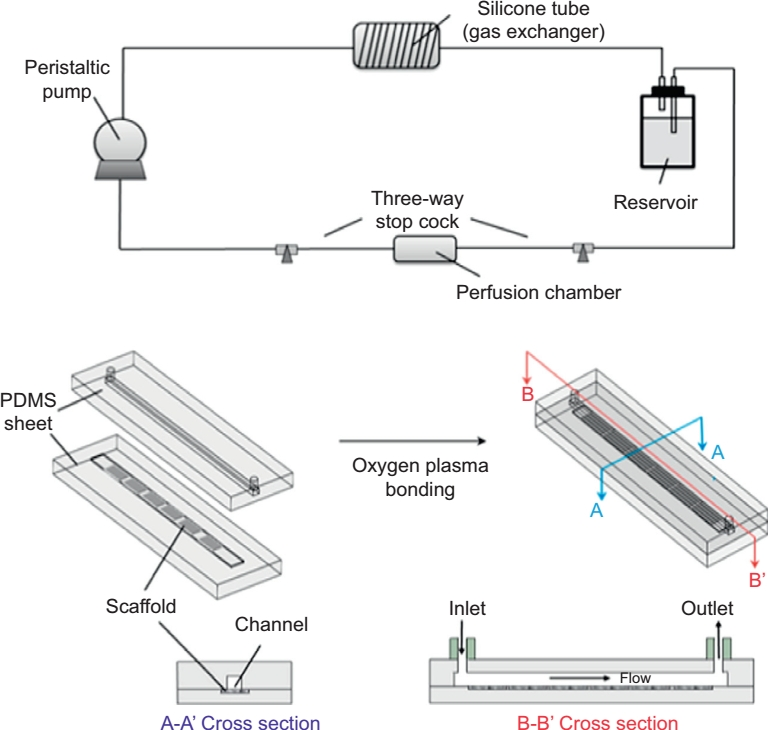
\includegraphics[width=0.85\textwidth]{mech_shear}
			
			\end{figure}
		\end{column}
	\end{columns}	
		

\end{frame}


\begin{frame}[fragile]{Pressure}  

		 	Schematic illustration of a cyclic pressure bioreactor.

			\begin{figure}
			\centering
			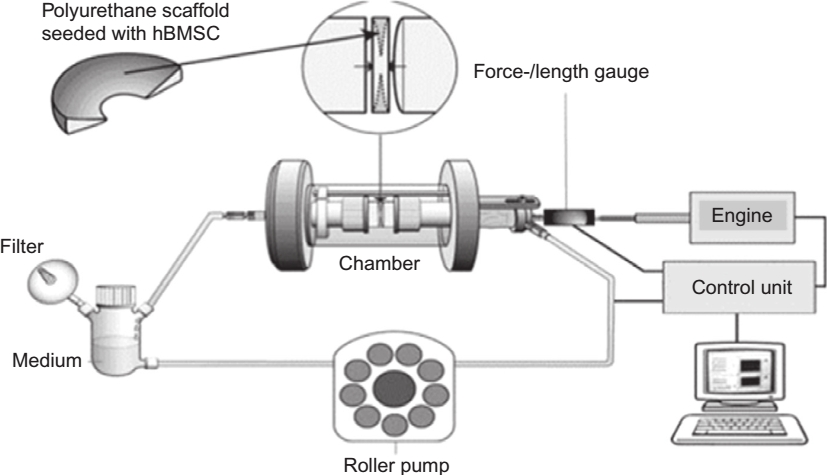
\includegraphics[width=0.57\textwidth]{mech_pressure}
			
			\end{figure}
	\footnotesize(K. J. Blosea et al., 2014)

\end{frame}


\begin{frame}[fragile]{Bending}  

		 	Schematic illustration of a cyclic bending bioreactor.

			\begin{figure}
			\centering
			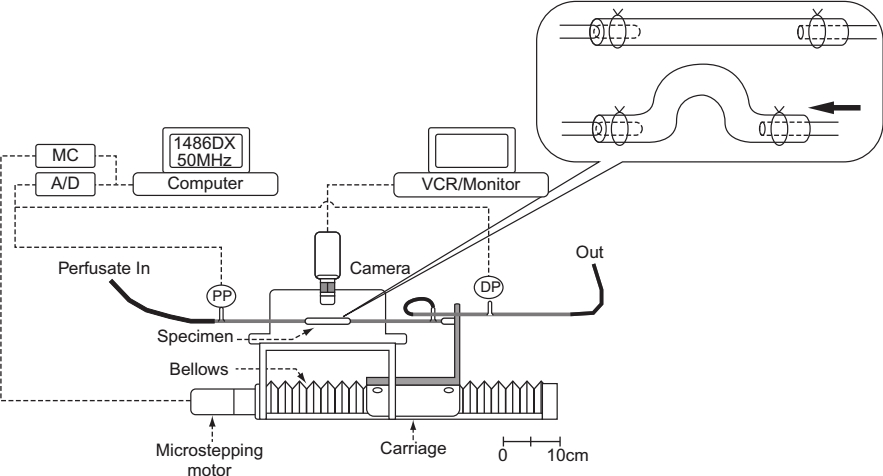
\includegraphics[width=0.57\textwidth]{mech_bending}
			
			\end{figure}
	\footnotesize(K. J. Blosea et al., 2014)

\end{frame}


\begin{frame}[fragile]{Different Types of Bioreactors}  

	\begin{columns}[t]
		\begin{column}{.45\textwidth}
		\begin{enumerate}[a.]
		\item
		Spinner flask
		\item
		Rotating-wall vessels 
		\item
		 Hollow-fiber
		\item
		Direct perfusion
		\item		
		Controlled mechanical forces 
		\end{enumerate}
		
		\vspace{50pt}
		\footnotesize(I. Martin et al., 2004)
 
		\end{column}
		\begin{column}{.55\textwidth}
			\vspace{-30pt}
			\begin{figure}
			\centering
			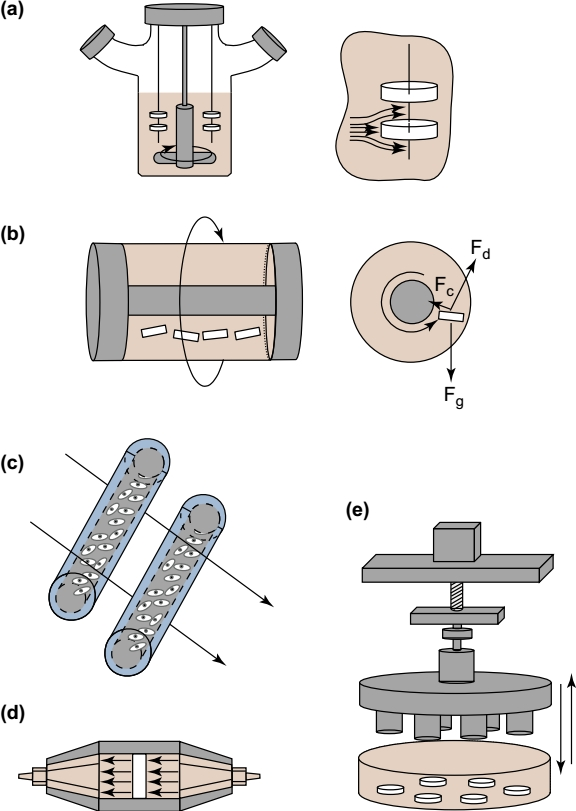
\includegraphics[width=0.6\textwidth]{types}
			
			\end{figure}
		\end{column}
	\end{columns}	
		
\end{frame}


\begin{frame}[fragile]{Features of Different Categories}  

\begin{itemize}
\item
Spinner flask bioreactors
\begin{itemize}
\item
Dynamic cell seeding
\item
Less control on the level of shear stress
\item
Manual waste removal
\item
Non-uniform velocity field
\end{itemize}
\item
Rotating-wall bioreactors  
\begin{itemize}
\item
High rate of mass transfer
\item
Relatively low shear stress conditions can be generated
\end{itemize}
\item
Perfusion bioreactors
\begin{itemize}
\item
Taking advantage of convective fluid flow but avoiding high levels of shear stress
\item
Effective seeding process and nutrient supply
\item
Automatic waste removal
\end{itemize}
\end{itemize}	
		
\end{frame}


\begin{frame}[fragile]{Scaffolds}  

Scaffolds fill critical roles in regenerative medicine:

\begin{enumerate}
\item
Provide anatomic fill and shape in
tissue defects
\item
Provide temporary function in anatomic
defects while tissue regenerates
\item
Enhance tissue regeneration through material-cell interaction and delivery of biologics, including cells, proteins, and/or genes
\end{enumerate}

\vfill
\footnotesize(S. J. Hollister, 2011)

		
\end{frame}


\begin{frame}[fragile]{Roles of Scaffolds - 4F}  

\begin{itemize}
\item
\textbf{F}orm:  Fill anatomic defect shape 
\item
\textbf{F}ixation: The mode of surgical fixation of the scaffold 
\item
\textbf{F}unction: Defining temporary function
\item
\textbf{F}ormation: Enhance tissue regeneration
\end{itemize}

\vfill
\footnotesize(S. J. Hollister, 2011)
		
\end{frame}


\begin{frame}[fragile]{Hierarchical Computational Scaffold Design}

 To compute scaffold structure-function relationships, 
 one should solve appropriate field equations at the architecture level:
 
 \begin{itemize}
 \item
 Effective elasticity $\rightarrow$ stress equilibrium
 \item
 Effective permeability $\rightarrow$ creeping Stokes fluid flow
 \item
 Effective diffusivity $\rightarrow$ local diffusivity
 \end{itemize}

	\begin{center}~
		\begin{beamercolorbox}[wd=.7\textwidth,sep=4pt,center]{box1}
		Finite Element Method (FEM)\\
		Computational Fluid Dynamics (CFD)\\
		Finite Difference Method (FDM)
		\end{beamercolorbox}
	\end{center}


\footnotesize(S. J. Hollister, 2011)
		
\end{frame}


\begin{frame}[fragile]{Effective Elasticity}
	
	Microstructural elasticity equation:
	\begin{gather*}
	\frac{\partial}{\partial x_j}E_{ijkl}\frac{\partial \chi^{pq}_k}{\partial x_l} = \frac{\partial}{\partial x_j}E_{ijpq}
	\end{gather*}
	
	$\rightarrow$ integration over the microstructure:
	\begin{gather*}
	E^{eff}_{ijkl} = \frac{1}{|V_{micro}|}\Int_{V_{micro}} E_{ijpq} \left( \delta_{kp}\delta_{lq}   - \frac{\partial \chi^{kl}_p}{\partial x_q} \right) dV_{micro}
	\end{gather*}

\vfill
\footnotesize(S. J. Hollister, 2011)
		
\end{frame}


\begin{frame}[fragile]{Effective diffusivity}
	
	Diffusion equation:
	\begin{gather*}
	\frac{\partial}{\partial x_i}D_{ij}\frac{\partial \chi^{p}}{\partial x_j} = \frac{\partial}{\partial x_i}D_{ip}
	\end{gather*}
	
	$\rightarrow$ integration over the microstructure:
	\begin{gather*}
	D^{eff}_{ij} = \frac{1}{|V_{micro}|}\Int_{V_{micro}} D_{ip} \left( \delta_{jp}   - \frac{\partial \chi^{j}}{\partial x_q} \right) dV_{micro}
	\end{gather*}

\vfill
\footnotesize(S. J. Hollister, 2011)
		
\end{frame}

\begin{frame}[fragile]{Effective permeability}
	
	Pressure gradient equation:
	\begin{gather*}
	\frac{\partial p^k}{\partial x_i}-\frac{\partial}{\partial x_j} \left( \frac{\partial v^{0k}_i}{x_j}   \right) = e^k_i
	\end{gather*}
	
	$\rightarrow$ integration over the microstructure:
	\begin{gather*}
	K^{eff}_{ik} = \frac{1}{\mu|V_{micro}|}\Int_{V_{micro}} v^{0k}_i dV_{micro}
	\end{gather*}

\vfill
\footnotesize(S. J. Hollister, 2011)
		
\end{frame}


\section{Design of Bioreactors}

\begin{frame}[fragile]{ Design Parameters of Flow Perfusion Bioreactors}

\begin{itemize}
\item
Direct Perfusion of Scaffolds
\item
Media Flow Pathway
\item
Maintenance of Sterility
\item
Environmental Control
\begin{itemize}
\item
Nutrient supply 
\item
Waste removal
\item
Gas exchange
\end{itemize}
\end{itemize}
	


\vfill
\footnotesize(E. J. Levorson et al., 2011)
		
\end{frame}


\begin{frame}[fragile]{Building a Simple Perfusion Bioreactor}

\textbf{Objective}:\\Design a perfusion bioreactor to employ circulatory flow throughout the system to provide
\begin{itemize}
\item
Sufficient nutrient transfer
\item
Removal of waste products
\item
Application of mechanical stimuli
\end{itemize}
	


\vfill
\footnotesize(J. Rosser et al., 2018)
		
\end{frame}


\begin{frame}[fragile]{Building a Simple Perfusion Bioreactor}  

	\begin{columns}[t]
		\begin{column}{.40\textwidth}
		\textbf{Components}:
		\begin{enumerate}
		\item
		a culture encasing bioreactor
		\item
		a vessel containing the oxygenated nutrient-rich medium 
		\item
		a pump capable of generating
flow throughout the system

		\end{enumerate}
		
		\vspace{10pt}
		\footnotesize(J. Rosser et al., 2018)
 
		\end{column}
		\begin{column}{.60\textwidth}
			%\vspace{-30pt}
			\begin{figure}
			\centering
			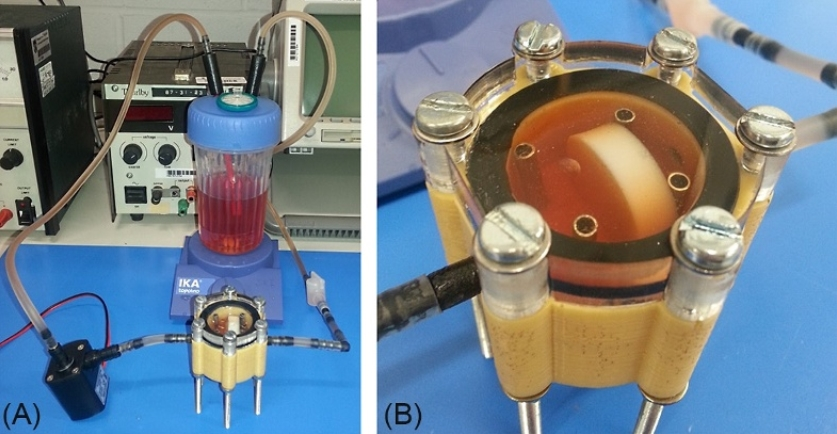
\includegraphics[width=0.9\textwidth]{design}
			
			\end{figure}
		\end{column}
	\end{columns}	
		
\end{frame}


\begin{frame}[fragile]{Taking Advantage of CFD}  

Using \textbf{CFD} to simulate fluid flow to obtain the optimum \emph{internal shape}, \emph{inlet/outlet positioning}, and \emph{scaffold fixture positioning}.
	
			\begin{figure}
			\centering
			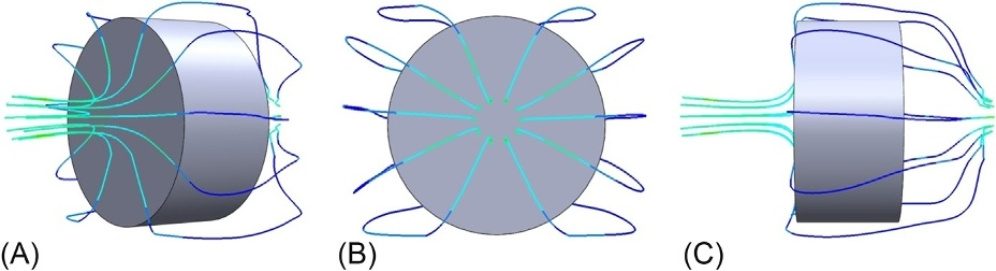
\includegraphics[width=0.8\textwidth]{design_cfd1}
			
			\vspace{10pt}			
			\footnotesize Flow trajectories around the vertical scaffold; (A) isometric, (B) front,
and (C) side views
			\end{figure}

\end{frame}

\begin{frame}[fragile]{Optimizing Inlet and Outlet}  

			\begin{figure}
			\centering
			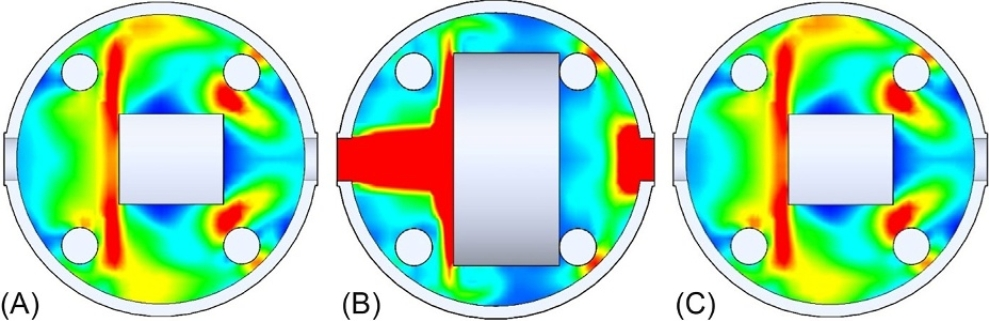
\includegraphics[width=0.8\textwidth]{design_cfd2}
			
			\vspace{15pt}
			\footnotesize (A) Lower, (B) middle, and (C) upper velocity contours with application-wide
scaffold supports
			\end{figure}

\end{frame}

\begin{frame}[fragile]{Bioreactor Base Design}  

			\begin{figure}
			\centering
			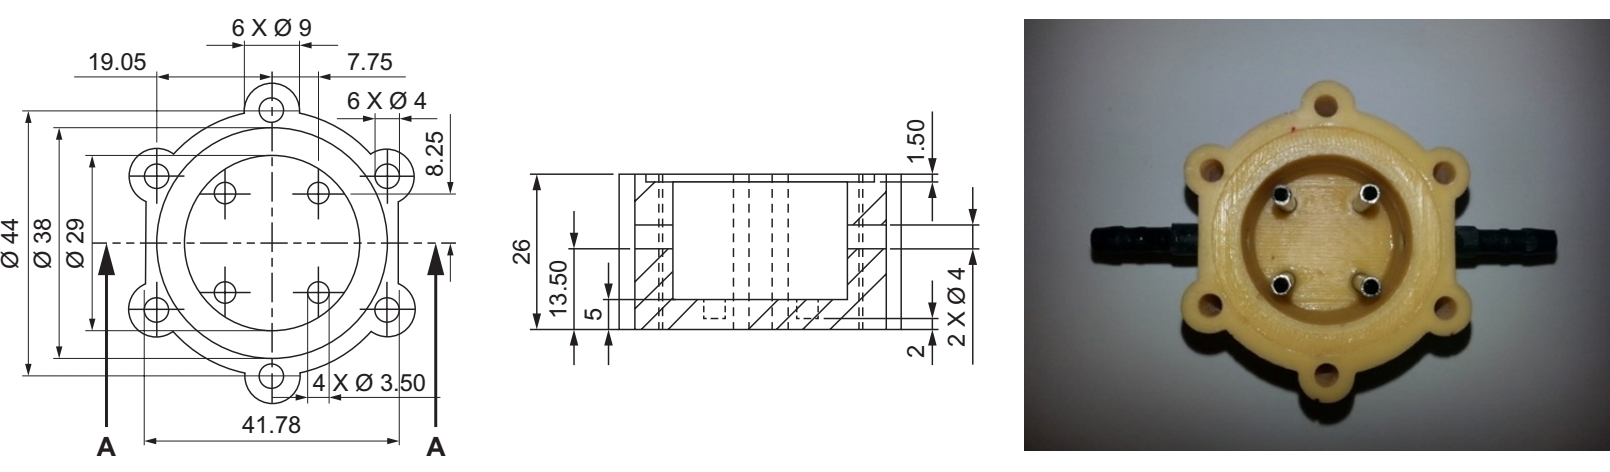
\includegraphics[width=0.9\textwidth]{design_base}
			
			\vspace{15pt}
			\footnotesize Bioreactor base dimensions (mm) and fully constructed bioreactor unit
			\end{figure}

\end{frame}


\begin{frame}[fragile]{Bioreactor Lid Design}  

			\begin{figure}
			\centering
			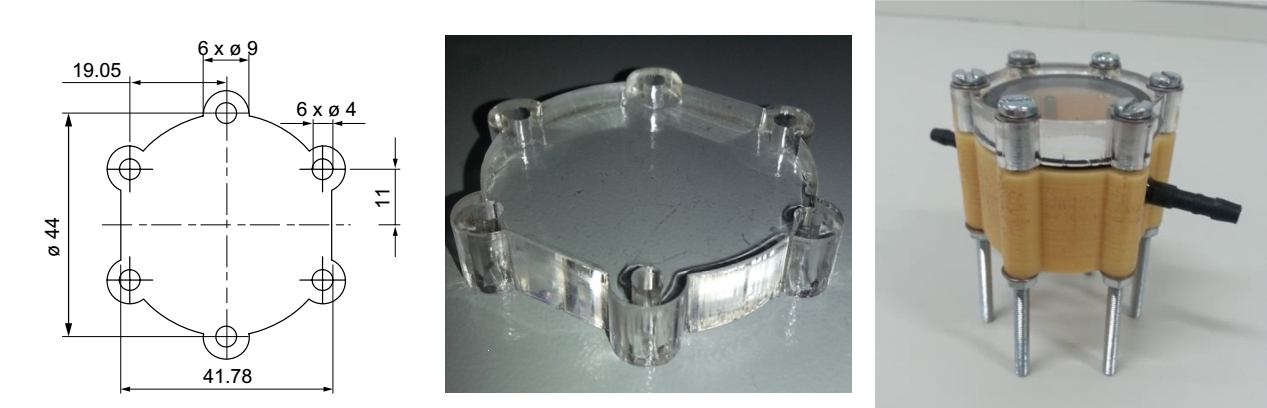
\includegraphics[width=0.9\textwidth]{design_lid}
			
			\vspace{15pt}
			\footnotesize Bioreactor lid dimensions (mm) and finished bioreactor base component
			\end{figure}

\end{frame}

\begin{frame}[fragile]{Medium Vessel Design}  

		\begin{columns}[t]
		\begin{column}{.50\textwidth}
					\vspace{50pt}
			\footnotesize Medium vessel dimensions (mm) and assembly 
 
		\end{column}
		\begin{column}{.50\textwidth}
			\vspace{-20pt}
			\begin{figure}
			\centering
			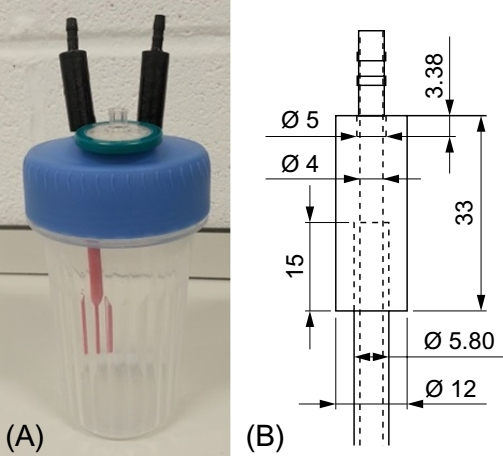
\includegraphics[width=0.9\textwidth]{design_medium}
			
			\end{figure}
		\end{column}
	\end{columns}

\end{frame}

\begin{frame}[fragile]{Pomp Design}  

			\begin{figure}
			\centering
			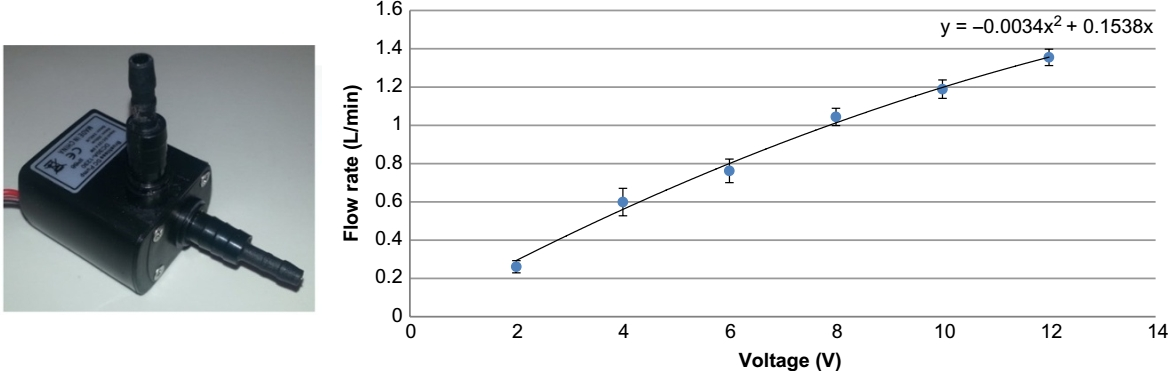
\includegraphics[width=0.9\textwidth]{design_pomp}
			
			\vspace{15pt}
			\footnotesize A 12V 4.8W 0.8A brushless DC pump and resulting flow rate values with specified voltages applied.
			\end{figure}

\end{frame}


\section{Bioreactor Modeling}

\begin{frame}[fragile]{Bioreactor Modeling}  

 Classification of nonlinear model forms used in bioreactor modeling
	
			\begin{figure}
			\centering
			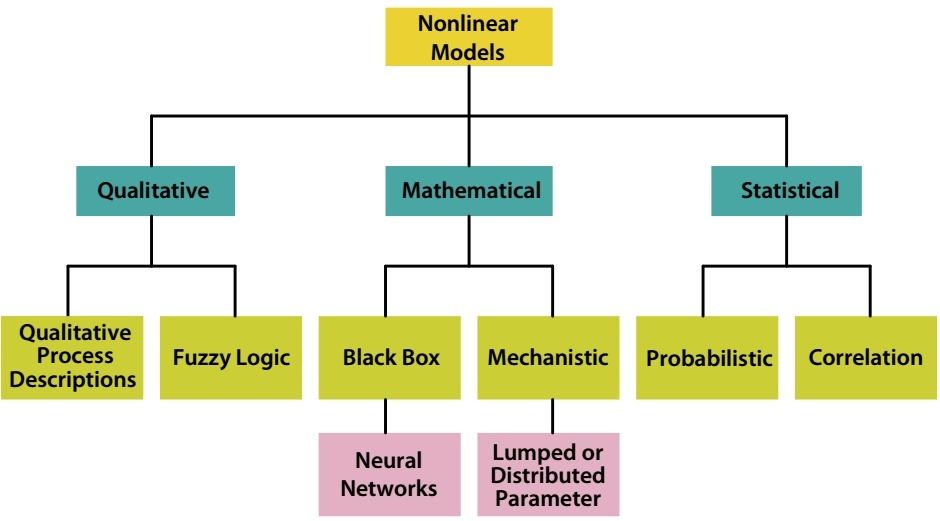
\includegraphics[width=0.68\textwidth]{models}			
			\footnotesize(C. Julien et al., 2007)
			\end{figure}
\end{frame}

\begin{frame}[fragile]{Mathematical Modeling of Bioreactors}  

 Mathematical modeling and simulation is essential to overcome the design challenges of Bioreactors.

\begin{exampleblock}{Examples of Mathematical Models}
\begin{itemize}
\item
Black Box Models:
\begin{itemize}
\item
Artificial Neural Networks
\item
Machine Learning-based Control
\end{itemize}
\item
Mechanistic (Conservative) Models
\begin{itemize}
\item
ODE - Ordinary Differential Equations
\item
PDE
 - Partial Differential Equations
\end{itemize}
\end{itemize}
\end{exampleblock}

\end{frame}


\begin{frame}[fragile]{Quantitative Models of Perfusion Bioreactors}

Investigating 2 Examples of Bioreactor Models:

\begin{itemize}
\item
\textbf{Example 1 (Simple Model)}:\\Modeling of the Flow within Scaffolds in Perfusion Bioreactors\\(X. Yan et al., 2011)
\item
\textbf{Example 2 (Complex Model)}:\\Mathematical Modeling of Three-Dimensional Cell Cultures in Perfusion Bioreactors\\(F. Coletti et al., 2006)
\end{itemize}

	\begin{center}~
		\begin{beamercolorbox}[wd=.8\textwidth,sep=4pt,center]{box1}
Materials similar to Example 2 are useful for students to be more familiar with the engineering aspects of Bioreactors. 
		\end{beamercolorbox}
	\end{center}

\end{frame}



\begin{frame}[fragile]{Example 1: Flow Model}

		\begin{columns}[t]
		\begin{column}{.45\textwidth}
			To control the cultivating process, the knowledge of the fluid flow
inside and around a scaffold in the bioreactor is essential.

\vspace{20pt}
Figure: Schematic of bioreactors: (a) perfusion bioreactor\\(b) non-perfusion bioreactor

\vspace{20pt}
\footnotesize(X. Yan et al., 2011)

		\end{column}
		\begin{column}{.55\textwidth}
			\vspace{-20pt}
			\begin{figure}
			\centering
			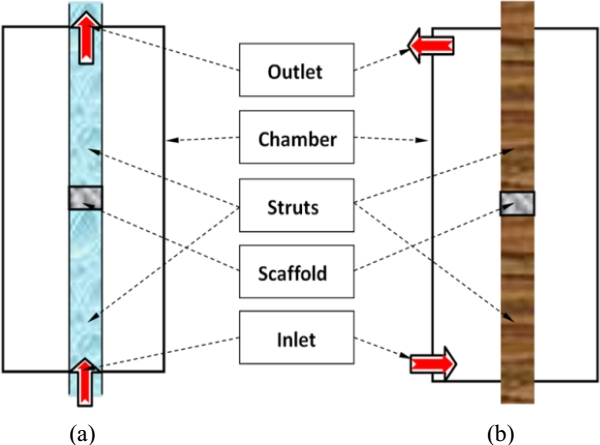
\includegraphics[width=0.9\textwidth]{flow_scheme}
			
			\end{figure}
		\end{column}
	\end{columns}

\end{frame}

\begin{frame}[fragile]{Scaffold Geometry}  

			\begin{figure}
			\centering
			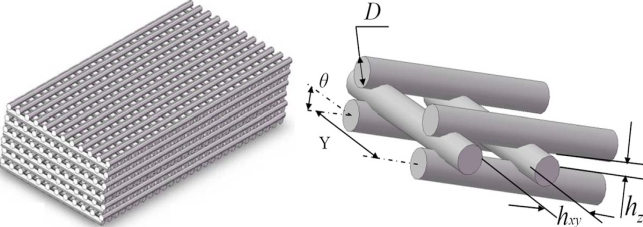
\includegraphics[width=0.75\textwidth]{flow_scaffold}
			
			\vspace{15pt}
			\footnotesize Geometric parameters for tissue scaffold
			\end{figure}

\end{frame}


\begin{frame}[fragile]{Model and Mesh Setup}  

	\begin{columns}[t]
		\begin{column}{.40\textwidth}
		\begin{enumerate}[a)]
		\item
		Final geometric model
		\item
		Mesh
		\item
		Refined mesh around tissue scaffold
		\end{enumerate}
	
 
		\end{column}
		\begin{column}{.60\textwidth}
			\vspace{-30pt}
			\begin{figure}
			\centering
			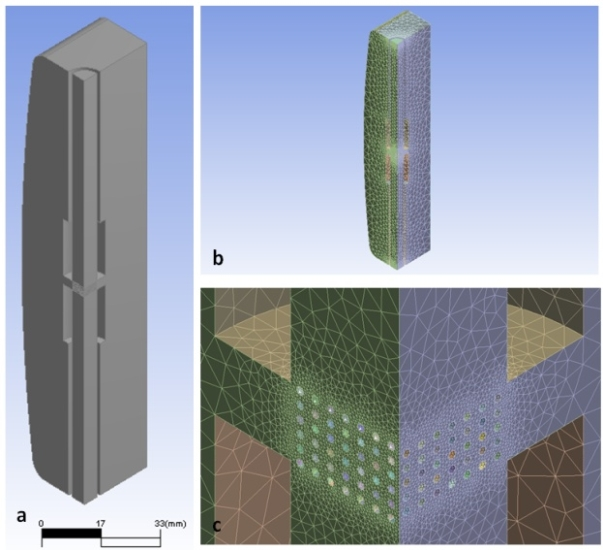
\includegraphics[width=0.8\textwidth]{flow_mesh}
			
			\end{figure}
		\end{column}
	\end{columns}	
		
\end{frame}


\begin{frame}[fragile]{Results: Perfusion Bioreactor}  

	\begin{columns}[t]
		\begin{column}{.40\textwidth}
		D=0.3mm and Y=0.7mm
		\begin{enumerate}[a)]
		\item
		Velocity streamlines in bioreactor
		\item
		Velocity streamlines around the tissue scaffold
		\item
		Surface shear stress distribution in the scaffold
		\end{enumerate}
	
 
		\end{column}
		\begin{column}{.60\textwidth}
			\vspace{-15pt}
			\begin{figure}
			\centering
			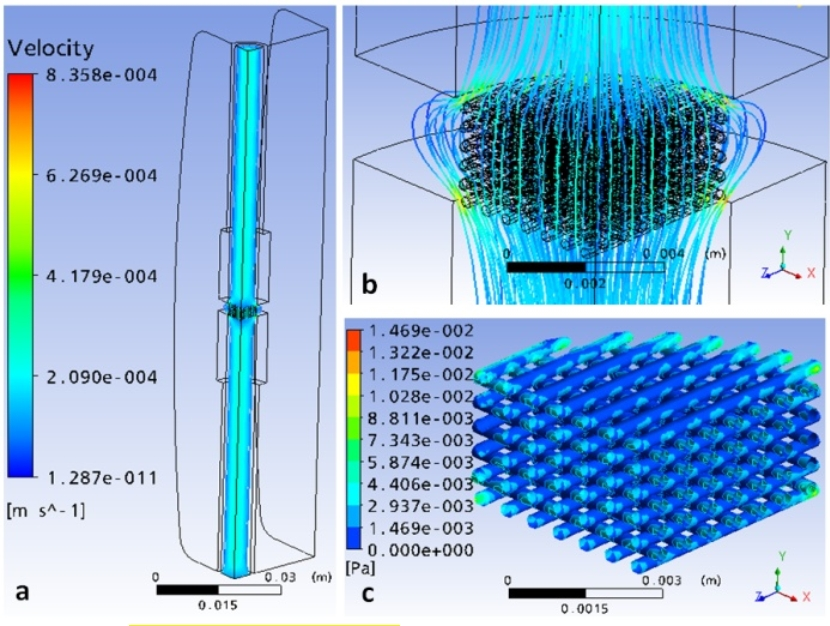
\includegraphics[width=0.8\textwidth]{flow_perf}
			
			\end{figure}
		\end{column}
	\end{columns}	
		
\end{frame}


\begin{frame}[fragile]{Results: Non-Perfusion Bioreactor}  

	\begin{columns}[t]
		\begin{column}{.40\textwidth}
		D=0.3mm and Y=0.7mm
		\begin{enumerate}[a)]
		\item
		Velocity streamlines in bioreactor
		\item
		Surface shear stress distribution in the scaffold
		\end{enumerate}
	
 
		\end{column}
		\begin{column}{.60\textwidth}
			\vspace{-15pt}
			\begin{figure}
			\centering
			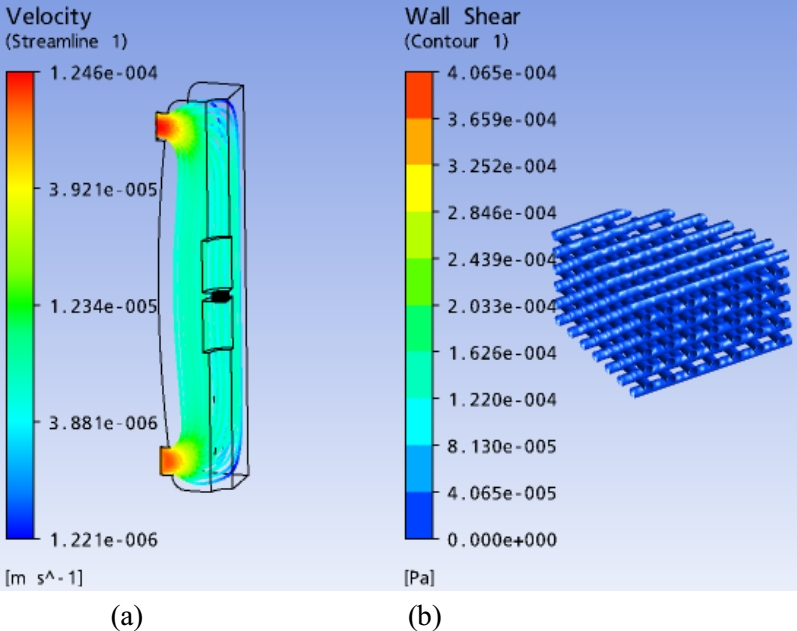
\includegraphics[width=0.8\textwidth]{flow_nonperf}
			
			\end{figure}
		\end{column}
	\end{columns}	
		
\end{frame}


\begin{frame}[fragile]{Results: Surface Shear Stress Distribution}  

			\begin{figure}
			\centering
			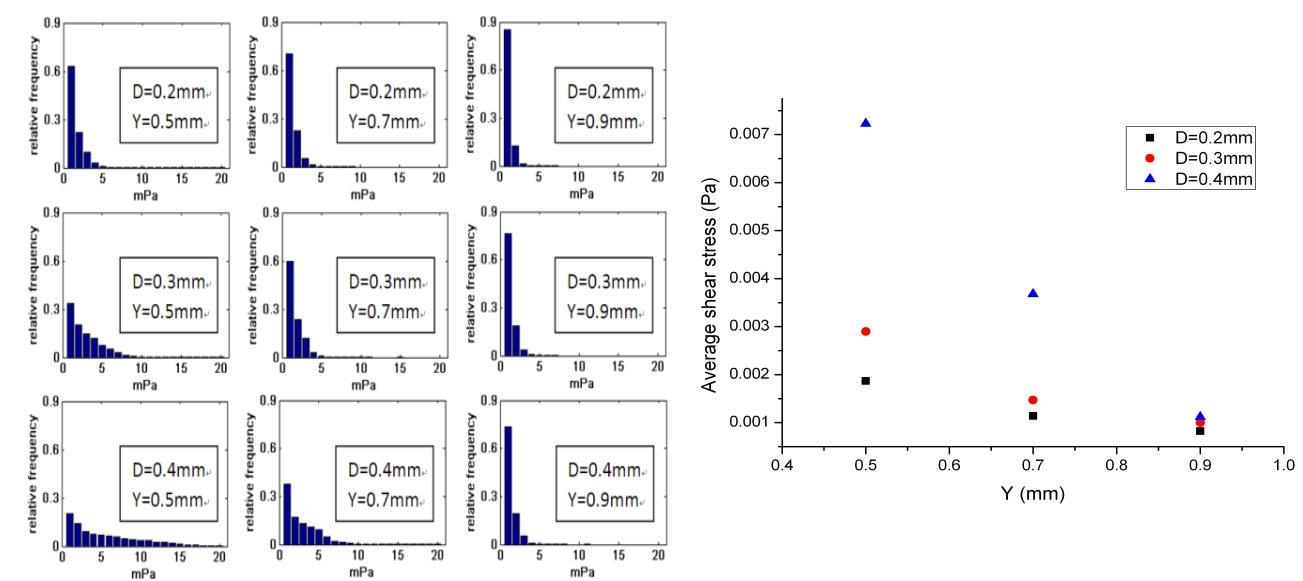
\includegraphics[width=0.8\textwidth]{flow_shear1}
			
			\vspace{5pt}
			\footnotesize Shear stress distribution versus D and Y
			\end{figure}

\end{frame}


\begin{frame}[fragile]{Results: Surface Shear Stress Distribution}  
\vspace{-10pt}
			\begin{figure}
			\centering
			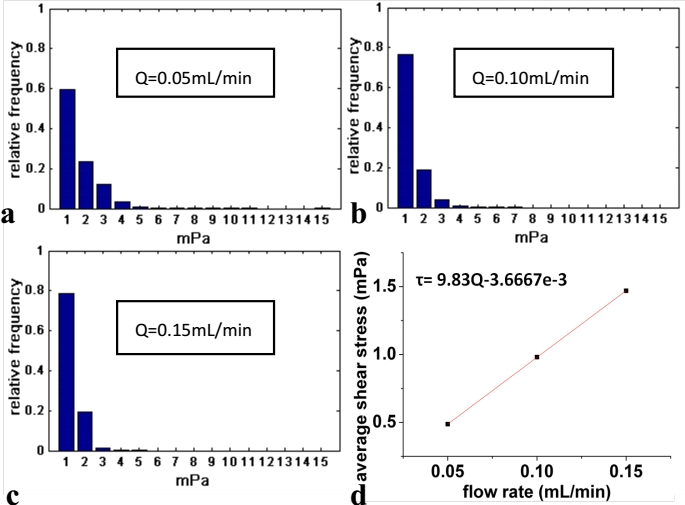
\includegraphics[width=0.55\textwidth]{flow_shear2}
			
			\vspace{5pt}
			\footnotesize  Shear stress distribution within scaffold for different flow rates
			\end{figure}

\end{frame}


\begin{frame}[fragile]{Example 2: Cell Cultures in Perfusion Bioreactor}  

Obtaining a proper oxygen supply, high cell density, and a uniform cell distribution in a 3D growth support are important challenges. 

\vspace{20pt}
$\xrightarrow{\text{To study all together}}$ Comprehensive mathematical model of perfusion bioreactor:
\begin{itemize}
\item
Fluid Flow
\item
Convection (Advection)
\item
Diffusion 
\item
Cell growth kinetics
\end{itemize}
\vfill
\footnotesize(F. Coletti et al., 2006)

\end{frame}

\begin{frame}[fragile]{Governing Equations}  

To model spatial-temporal evolution of \textit{oxygen concentration} and \textit{cell density} within a 3D polymeric scaffold:

\begin{itemize}
\item
Flow inside the bioreactor $\rightarrow$ Navier-Stokes equations
\item
Convection through the scaffold $\rightarrow$ Brinkman’s extension of Darcy’s law
\item
The oxygen uptake rate $\rightarrow$ Michaelis-Menten kinetics
\item
Cell growth $\rightarrow$ Function of oxygen concentration in the Contois equation
\end{itemize}

\end{frame}

\begin{frame}[fragile]{Conceptual Model}  

	\begin{columns}[t]
		\begin{column}{.40\textwidth}
Schematic demonstration of the main interacting phenomena that occur in a perfusion bioreactor when convective and diffusive flux and cell proliferation take place within the scaffold
	
 
		\end{column}
		\begin{column}{.60\textwidth}
			\vspace{-20pt}
			\begin{figure}
			\centering
			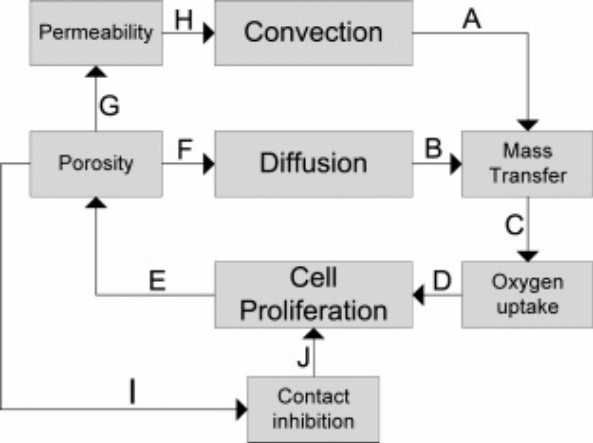
\includegraphics[width=0.8\textwidth]{math_scheme}
			
			\end{figure}
		\end{column}
	\end{columns}	
		
\end{frame}


\begin{frame}[fragile]{Line A}  

	\begin{columns}[t]
		\begin{column}{.75\textwidth}
Momentum balance by the Navier-Stokes equations
\[
\rho \frac { \partial \vec { v } ^ { 0 } } { \partial t } + \rho \left( \vec { v } ^ { 0 } \cdot \nabla \right) \vec { v } ^ { 0 } = - \nabla P + \mu \nabla ^ { 2 } \vec { v } ^ { 0 } + \rho \vec { g }
\]
Continuity equation for incompressible fluid
\[
\nabla \vec { v } ^ { 0 } = \frac { \partial v _ { z } ^ { 0 } } { \partial z } + \frac { 1 } { r } \frac { \partial r v _ { r } ^ { 0 } } { \partial r } + \frac { 1 } { r } \frac { \partial v _ { \vartheta } ^ { 0 } } { \partial \vartheta } = 0
\]
Brinkman’s extension to Darcy’s law for porous media
\[
\rho \frac { \partial \vec { v } } { \partial t } = - \nabla P - \frac { \mu } { K } \vec { v } + \mu \nabla ^ { 2 } \vec { v } + \rho \vec { g }
\]


		\end{column}
		\begin{column}{.25\textwidth}
			
			\begin{figure}
			\centering
			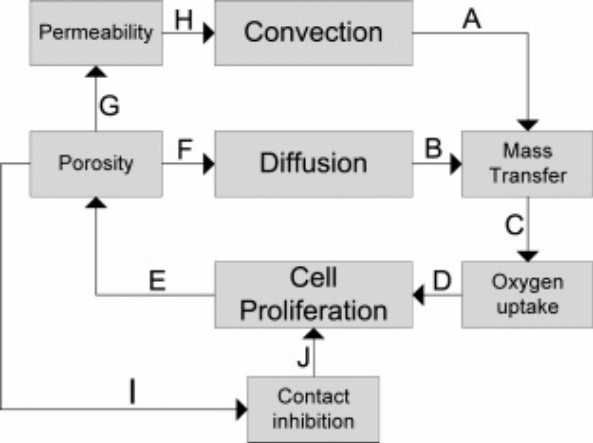
\includegraphics[width=\textwidth]{math_scheme}
			
			\end{figure}
		\end{column}
	\end{columns}	
		
\end{frame}


\begin{frame}[fragile]{Line B}  

	\begin{columns}[t]
		\begin{column}{.75\textwidth}
Species mass balance that includes convective and diffusion terms
\[
\frac { \partial c _ { i } } { \partial t } = - \left( \nabla \cdot c _ { i } \vec { v } ^ { 0 } \right) + \nabla \cdot \left( D _ { i } \nabla c _ { i } \right)
\]
Material balance in the scaffold
\[
\frac { \partial c _ { i } } { \partial t } = - \left( \nabla \cdot c _ { i } \vec { v } \right) + \nabla \cdot \left( D _ { \mathrm { eff } _ { i } } \nabla c _ { i } \right) + R _ { i }
\]

		\end{column}
		\begin{column}{.25\textwidth}
			
			\begin{figure}
			\centering
			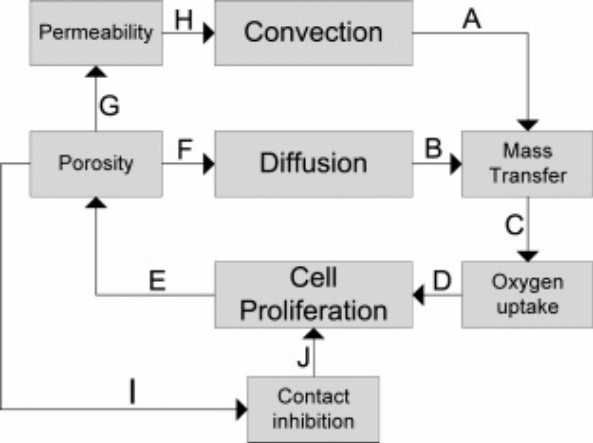
\includegraphics[width=\textwidth]{math_scheme}
			
			\end{figure}
		\end{column}
	\end{columns}	
		
\end{frame}

\begin{frame}[fragile]{Line C and D}  

	\begin{columns}[t]
		\begin{column}{.75\textwidth}
\textbf{Line C}: Reaction rate expressed in the form of Michaelis-Menten kinetics
\[
R _ { \mathrm { O } _ { 2 } } = \rho _ { \mathrm { cell } } \frac { Q _ { \mathrm { m } } c _ { \mathrm { O } _ { 2 } } } { C _ { \mathrm { m } } + c _ { \mathrm { O } _ { 2 } } }
\]
\textbf{Line D}: The cell density
variation with respect to time
\[
\frac { \partial \rho _ { \mathrm { cell } } } { \partial t } = \left( \frac { \mu _ { \mathrm { cell } } ^ { \max } c _ { i } } { K _ { \mathrm { c } } \rho _ { \mathrm { cell } } V _ { \mathrm { cell } } \rho _ { c } + c _ { i } } - k _ { d } \right) \rho _ { \mathrm { cell } }
\]

		\end{column}
		\begin{column}{.25\textwidth}
			
			\begin{figure}
			\centering
			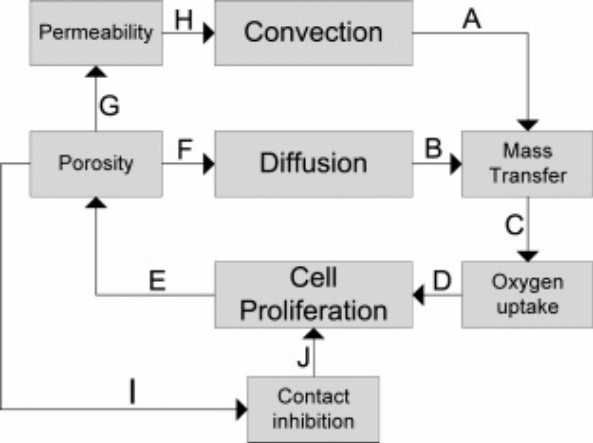
\includegraphics[width=\textwidth]{math_scheme}
			
			\end{figure}
		\end{column}
	\end{columns}	
		
\end{frame}

\begin{frame}[fragile]{Line E and F}  

	\begin{columns}[t]
		\begin{column}{.75\textwidth}
\textbf{Line E}: Reduction in scaffold porosity
\[
\epsilon ( z , r , t ) = \epsilon ( z , r , 0 ) - V _ { \text { cell } } \rho _ { \text { cell } } ( z , r , t )
\]
\textbf{Line F}: Effective diffusion coefficient as a function of porosity and tortuosity
\[
D _ { \mathrm { eff } } ( z , r , t ) = \frac { \epsilon ( z , r , t ) } { \tau ( z , r , t ) } D
\]

		\end{column}
		\begin{column}{.25\textwidth}
			
			\begin{figure}
			\centering
			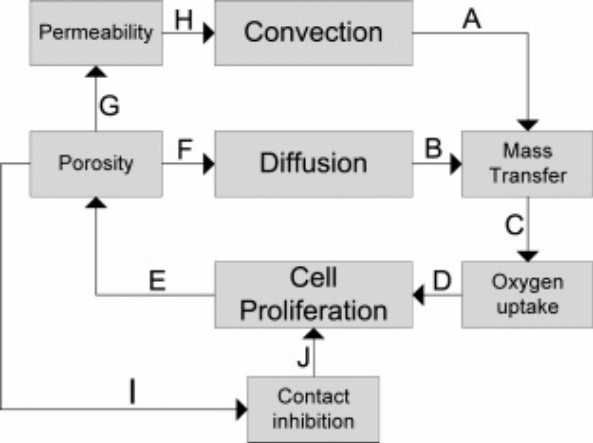
\includegraphics[width=\textwidth]{math_scheme}
			
			\end{figure}
		\end{column}
	\end{columns}	
		
\end{frame}

\begin{frame}[fragile]{Line G and H}  

	\begin{columns}[t]
		\begin{column}{.75\textwidth}
\textbf{Line G}: Tortuosity is modeled as a function of porosity
\[
\tau = \left( \frac { 2 - \epsilon } { \epsilon } \right) ^ { 2 }
\]
\textbf{Line H}: The functional form of Koponen is used for permeability
\[
K = \frac { \epsilon ^ { 3 } } { \mathrm { q } \tau ^ { 2 } s ^ { 2 } }
\]

		\end{column}
		\begin{column}{.25\textwidth}
			
			\begin{figure}
			\centering
			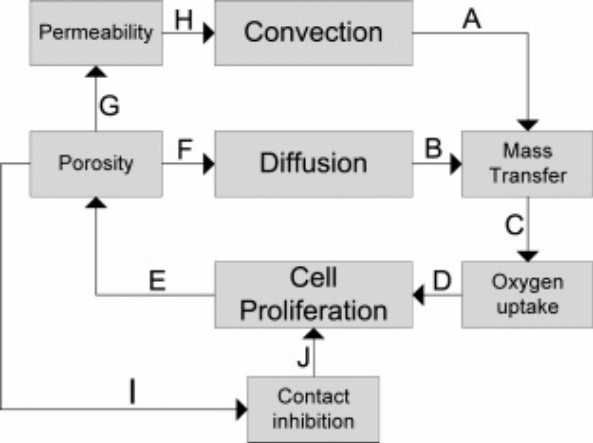
\includegraphics[width=\textwidth]{math_scheme}
			
			\end{figure}
		\end{column}
	\end{columns}	
		
\end{frame}

\begin{frame}[fragile]{Line I and J}  

	\begin{columns}[t]
		\begin{column}{.75\textwidth}
\textbf{Line I}: The Contois equation  to describe cell growth
\[
\mu _ { \mathrm { cell } } = \frac { \mu _ { \mathrm { cell } } ^ { \max } c _ { i } } { K _ { \mathrm { c } } \rho _ { \mathrm { cell } } V _ { \mathrm { cell } } \rho _ { \mathrm { c } } + c _ { i } }
\]
\textbf{Line J}: Similar to Line D
\[
\frac { \partial \rho _ { \mathrm { cell } } } { \partial t } = \left( \frac { \mu _ { \mathrm { cell } } ^ { \max } c _ { i } } { K _ { \mathrm { c } } \rho _ { \mathrm { cell } } V _ { \mathrm { cell } } \rho _ { c } + c _ { i } } - k _ { d } \right) \rho _ { \mathrm { cell } }
\]
		\end{column}
		\begin{column}{.25\textwidth}
			
			\begin{figure}
			\centering
			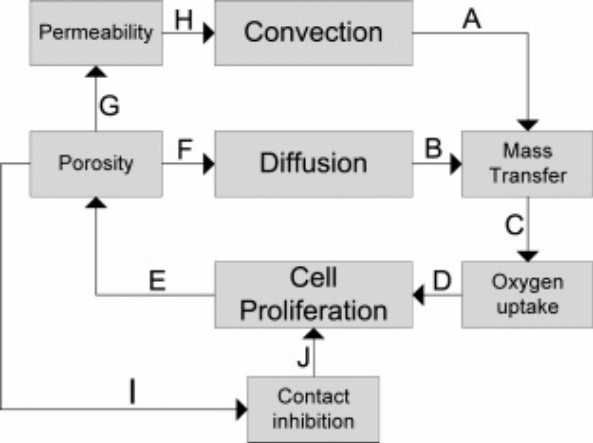
\includegraphics[width=\textwidth]{math_scheme}
			
			\end{figure}
		\end{column}
	\end{columns}	
		
\end{frame}


\begin{frame}[fragile]{Simulating the Model}  

The model is used to simulate two conditions:

\begin{itemize}
\item
\textbf{Case 1}: Total flow perfusion (left)
\item
\textbf{Case 2}: Partial flow perfusion with flow channelling at the walls (right)
\end{itemize}

			\begin{figure}
			\centering
			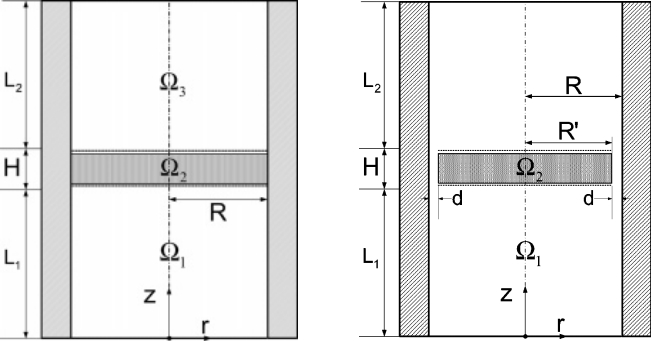
\includegraphics[width=0.50\textwidth]{math_models}
			\end{figure}

\end{frame}




\begin{frame}[fragile]{Results: Case 1, Total  Flow Perfusion}  
			
			\begin{figure}
			\centering
			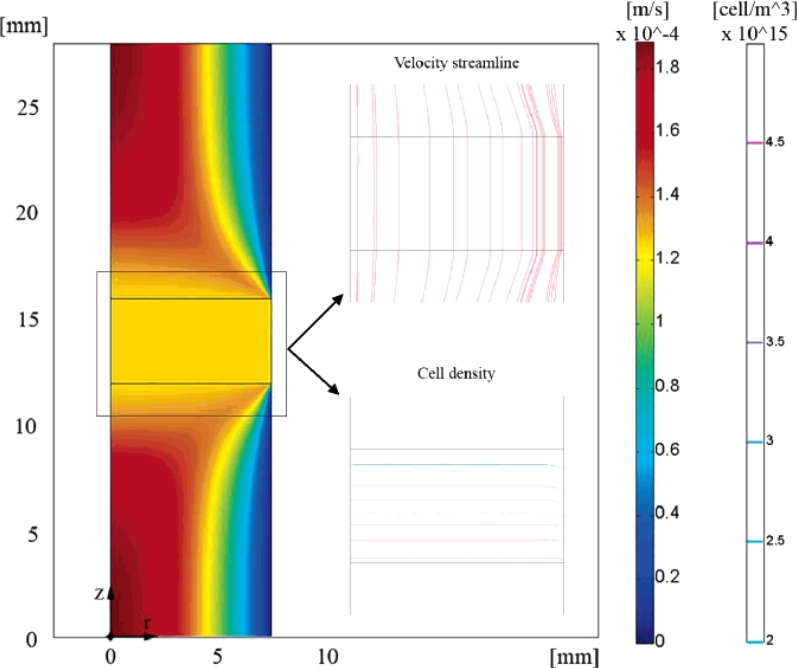
\includegraphics[width=0.5\textwidth]{math_tot_vel}
			
			\end{figure}
		
\end{frame}

\begin{frame}[fragile]{Results: Cell Density}  

	\begin{columns}[t]
		\begin{column}{.5\textwidth}
 Cell density in the scaffold on a logarithmic scale at 1-7 culture days  (a) and for the last 3 culture days (b).
	
 
		\end{column}
		\begin{column}{.5\textwidth}
			\vspace{-45pt}
			\begin{figure}
			\centering
			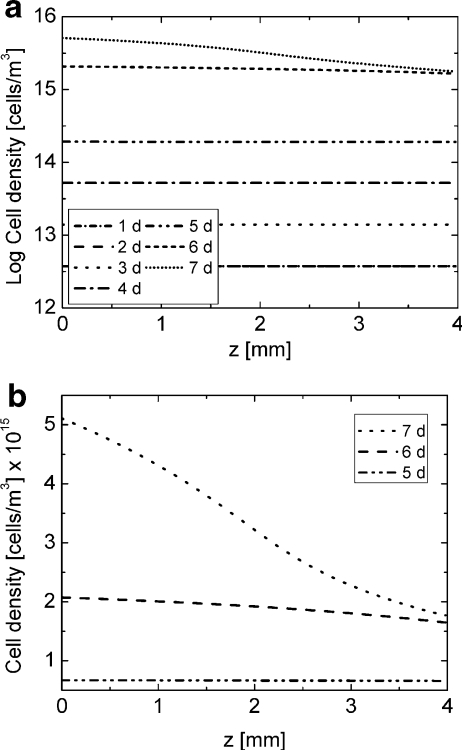
\includegraphics[width=0.6\textwidth]{math_tot_cell}
			
			\end{figure}
		\end{column}
	\end{columns}	
		
\end{frame}


\begin{frame}[fragile]{Results: Oxygen Concentration}  

	\begin{columns}[t]
		\begin{column}{.5\textwidth}
Oxygen concentration in the medium fluid within the scaffold after 1-7 culture days. Between the 5th and the 6th day, the oxygen concentration decreases to values lower than the minimum value for cell
viability indicated by the horizontal line
	
 
		\end{column}
		\begin{column}{.5\textwidth}
			\vspace{-5pt}
			\begin{figure}
			\centering
			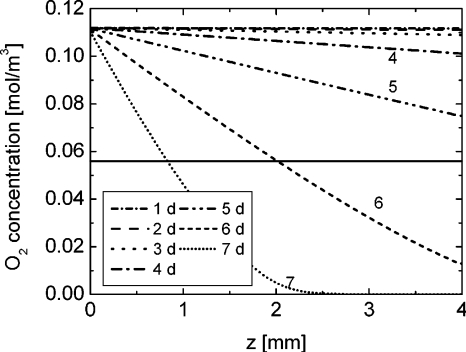
\includegraphics[width=0.7\textwidth]{math_tot_oxy}
			
			\end{figure}
		\end{column}
	\end{columns}	
		
\end{frame}


\begin{frame}[fragile]{Results: Cell and Oxygen Density}  

	\begin{columns}[t]
		\begin{column}{.5\textwidth}
 Oxygen (a) and cell density (b) profiles within the scaffold domain after 7 culture days, for several oxygen concentrations in the medium inlet fluid
	
 
		\end{column}
		\begin{column}{.5\textwidth}
			\vspace{-30pt}
			\begin{figure}
			\centering
			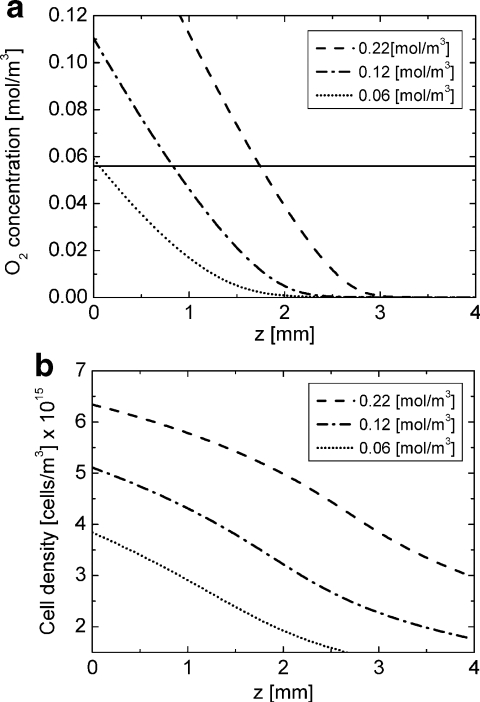
\includegraphics[width=0.6\textwidth]{math_tot_den}
			
			\end{figure}
		\end{column}
	\end{columns}	
		
\end{frame}

\begin{frame}[fragile]{Results: Effect of Flow Rate}  

	\begin{columns}[t]
		\begin{column}{.5\textwidth}
Effect of medium flow rate on oxygen profiles (a) and cell density (b) within the scaffold at day 7
	
 
		\end{column}
		\begin{column}{.5\textwidth}
			\vspace{-30pt}
			\begin{figure}
			\centering
			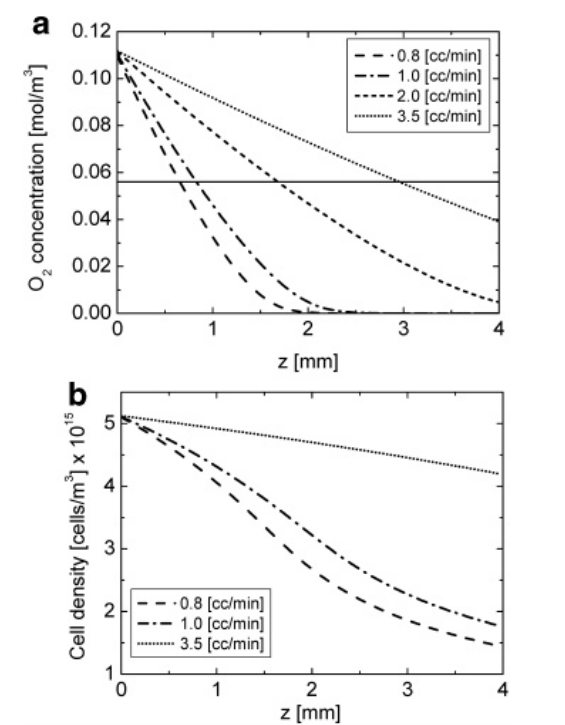
\includegraphics[width=0.7\textwidth]{math_tot_flow}
			
			\end{figure}
		\end{column}
	\end{columns}	
		
\end{frame}


\begin{frame}[fragile]{Results: Case 1, Partial  Flow Perfusion}  
			
			\begin{figure}
			\centering
			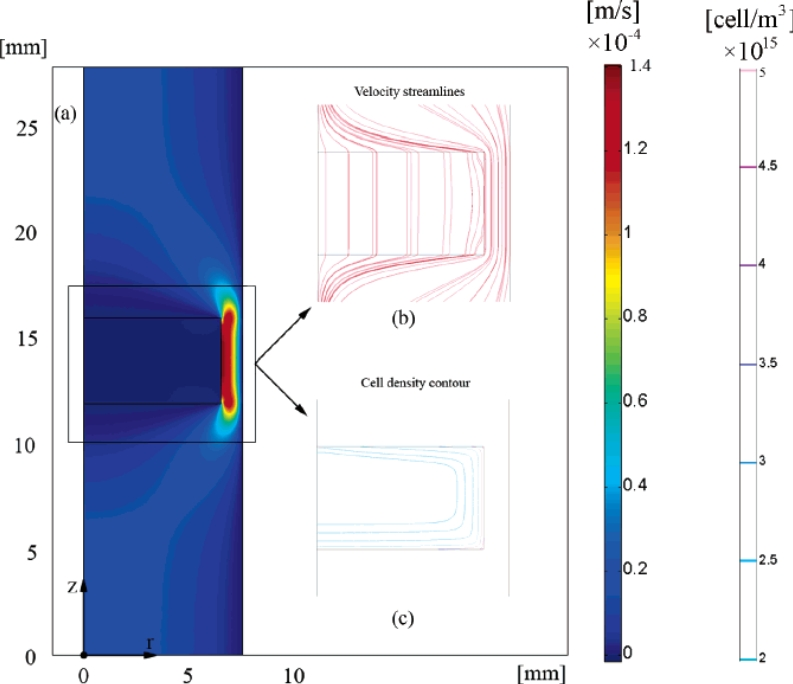
\includegraphics[width=0.5\textwidth]{math_par_vel}
			
			\end{figure}
\end{frame}


\begin{frame}[fragile]{Results: Comparison of Cell Density}  

	\begin{columns}[t]
		\begin{column}{.5\textwidth}
Cell density after 7 days within the scaffold for total (d = 0)
and partial perfusion (d > 0) with different channel gaps d, at 4 mm from
the scaffold center. When the channel gap (d) is only 0.1 mm, the effect on
cell distribution is quite small while the cell distribution differs significantly
from the total perfusion case for (d > 1 mm)
	
 
		\end{column}
		\begin{column}{.5\textwidth}
			\begin{figure}
			\centering
			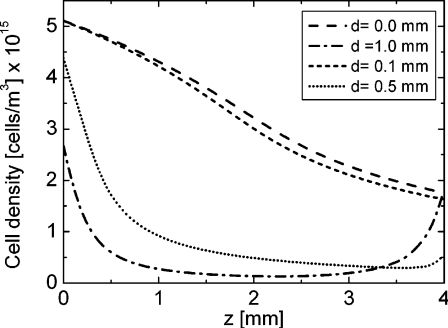
\includegraphics[width=0.7\textwidth]{math_comp1}
			
			\end{figure}
		\end{column}
	\end{columns}	
		
\end{frame}


\begin{frame}[fragile]{Results: Comparison of Cell Density}  

	\begin{columns}[t]
		\begin{column}{.4\textwidth}
Cell density contours after 7 days of culture in a section at 4 mm from the scaffold center in the case of total perfusion (a) and partial perfusion
with\\ d = 0.1 (b), \\d = 0.5 (c), \\and d = 1 mm (d).\\The greater the channel gap, the lower the cell density obtained.
	
 
		\end{column}
		\begin{column}{.6\textwidth}
			\vspace{-25pt}
			\begin{figure}
			\centering
			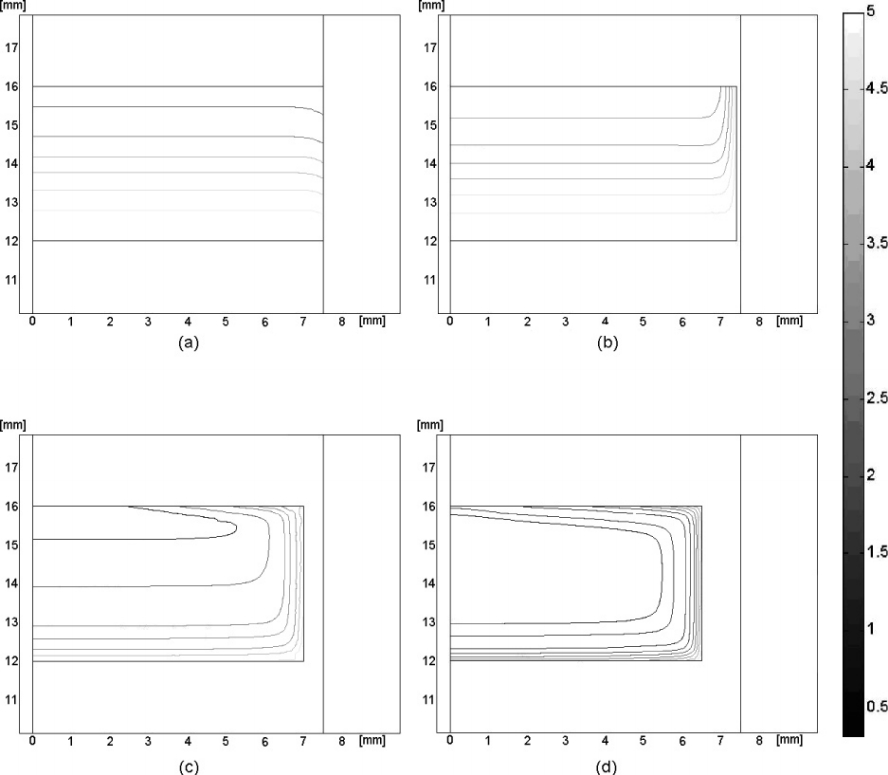
\includegraphics[width=0.85\textwidth]{math_comp2}
			
			\end{figure}
		\end{column}
	\end{columns}	
		
\end{frame}

\begin{frame}[fragile]{Example 2: Conclusion}  

	The two cases illustrated, total and partial perfusion, represent situations where the dominant oxygen transfer mechanism changes from being essentially convective, when no channelling is present, to essentially diffusive, when large channelling gaps
occur near the wall.

	\begin{center}~
		\begin{beamercolorbox}[wd=.7\textwidth,sep=4pt,center]{box1}
Although this example is relatively complex for students, it is suitable for teaching the concepts of diffusion and convection in Bioreactors and how they affect Tissue Engineering products.
		\end{beamercolorbox}
	\end{center}
	
	\begin{center}~
		\begin{beamercolorbox}[wd=0.8\textwidth,sep=4pt,center]{box2}	
		We can overcome the complexity of this example using an\\ \textbf{effective educational tool}!
		\end{beamercolorbox}
	\end{center}
		
\end{frame}


\section{Utilizing Jupyter Notebooks}


\begin{frame}[fragile]{Jupyter}  
			
			Project Jupyter exists to develop open-source software, open-standards, and services for \textbf{interactive computing} across dozens of programming languages.

			\begin{figure}
			\centering
			
\includegraphics[width=0.7\textwidth]{jupyter}
			
			\end{figure}
\end{frame}

\begin{frame}[fragile]{Why Jupyter Is Important?}

	\begin{block}{Jupyter}
	Considered as a \textbf{game-changer for research} because it enables scientific researchers to share detailed descriptions of raw code that then allow others to validate and build on their research.
	\end{block}  

 
	\begin{block}{Jupyter Notebooks}
The computational notebooks are described as the computing equivalent of a scientist’s lab notebook -- an environment in which scientists worldwide can develop code and run it immediately in their notebook environment.
	\end{block}  
	
\end{frame}

\begin{frame}[fragile]{Why Using Jupyter Notebooks in Education?}  

Jupyter Notebooks

\begin{itemize}
\item
Make learning in the class active and interactive
\item
Eliminate the complexity of getting started
\item
Facilitate rapid iteration and hence faster learning.
\item
Allow embedding of support content (image, video, formula, text, links) right next to code
\item
Can be used for creating interactive assignments (even auto-graded!)
\end{itemize}

\end{frame}

\begin{frame}[fragile]{Why Using Jupyter Notebooks in Education?}
			
			\begin{figure}
			\centering
			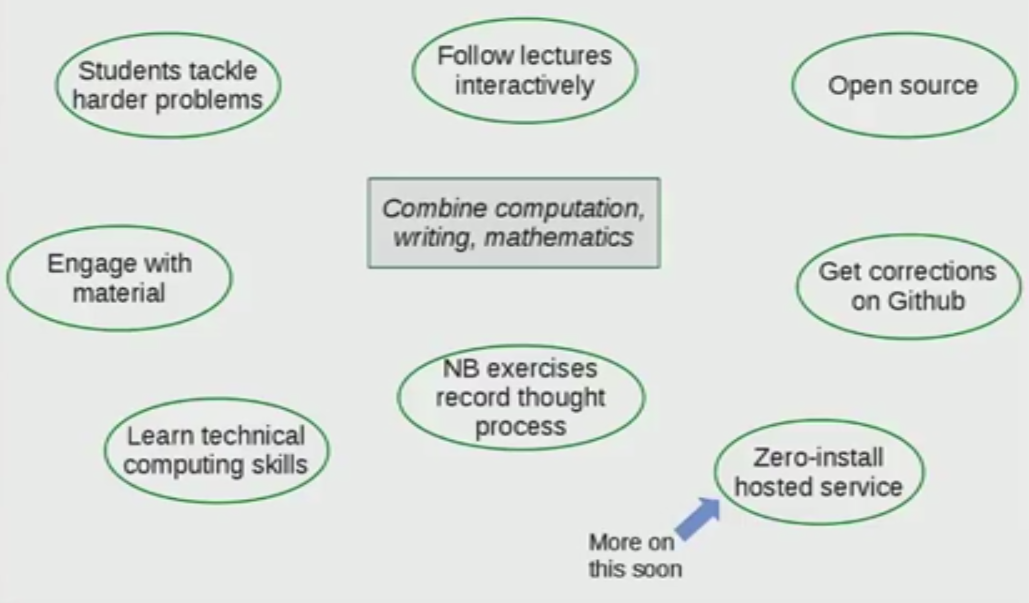
\includegraphics[width=0.65\textwidth]{jupyter_why}
			
			\vspace{5pt}
			\footnotesize (EuroPython 2017,  Jupyter notebooks for teaching and learning [\href{https://av.tib.eu/media/33805}{Link to video}])
			
			\end{figure}
\end{frame}

\begin{frame}[fragile]{Examples}  

	\begin{columns}[t]
		\begin{column}{.3\textwidth}
		Jupyter Notebooks powering UC Berkeley’s classes
	
 
		\end{column}
		\begin{column}{.7\textwidth}
			\vspace{-25pt}
			\begin{figure}
			\centering
			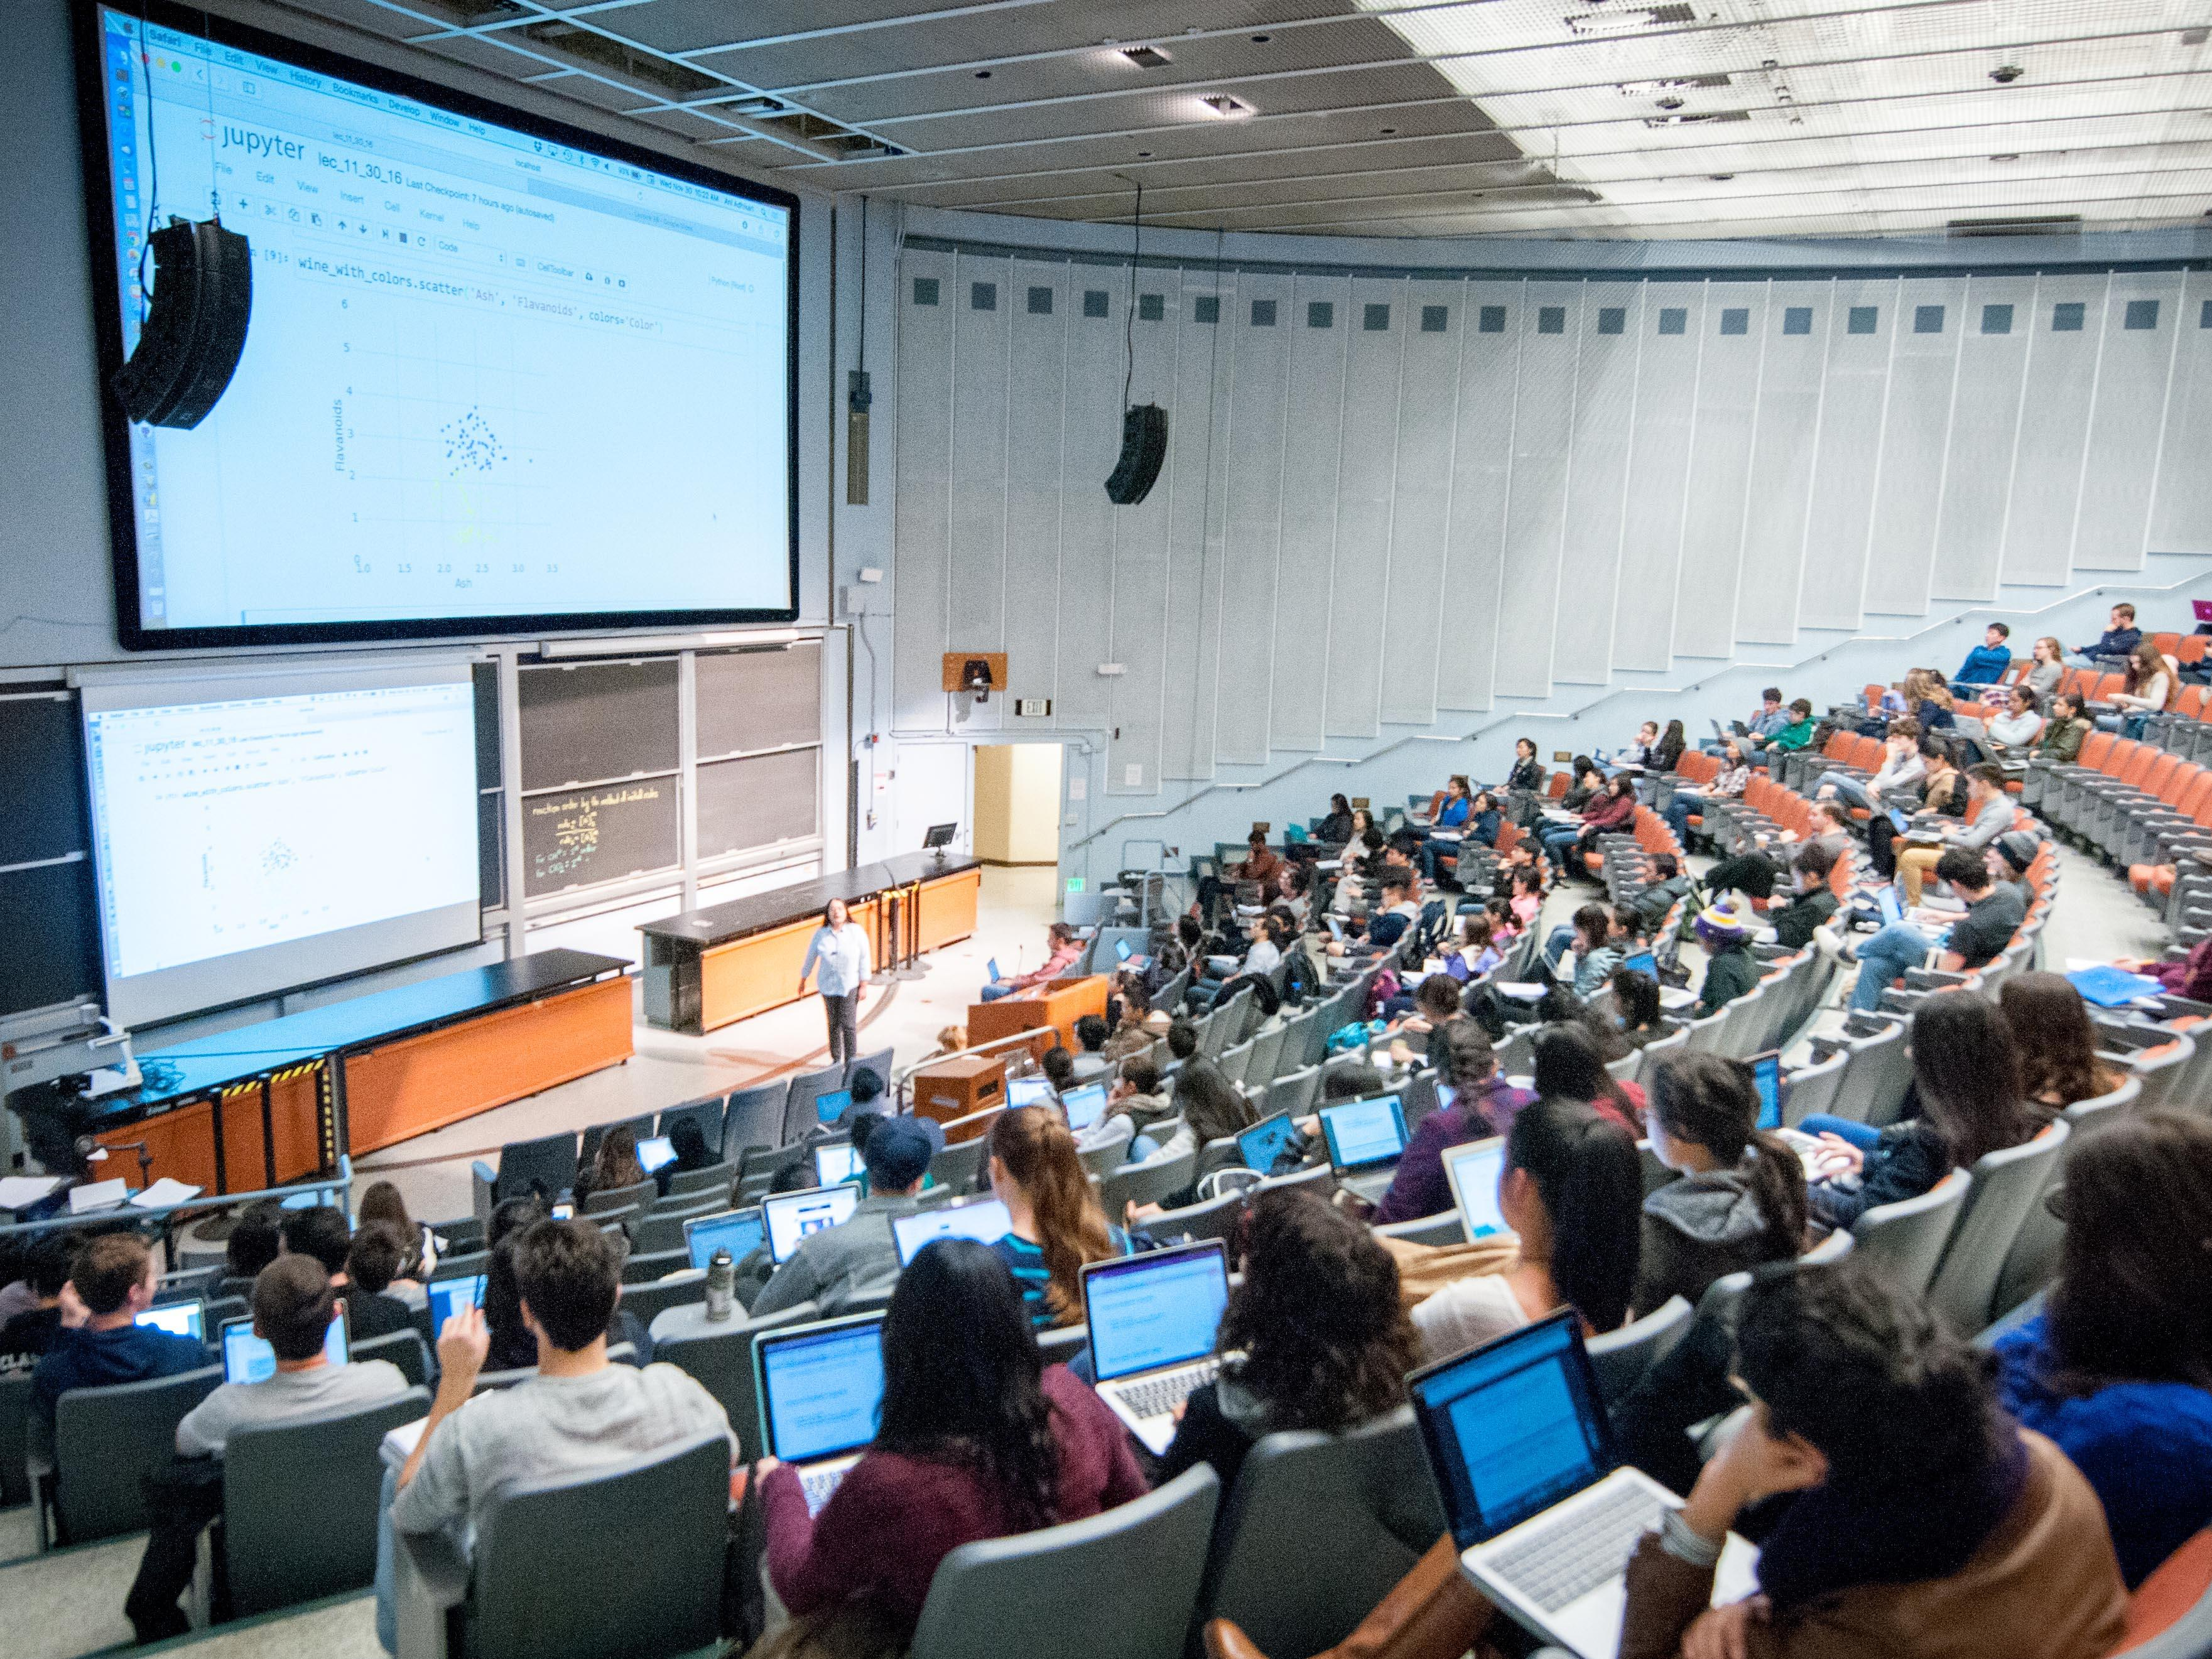
\includegraphics[width=0.85\textwidth]{jupyter_berkeley}
			
			\end{figure}
		\end{column}
	\end{columns}	
		
\end{frame}


\begin{frame}[fragile]{Examples}  

	\begin{columns}[t]
		\begin{column}{.3\textwidth}
		A well-known powerful CFD course by taking advantage of Jupyter Notebooks [\href{https://github.com/barbagroup/CFDPython}{Link}]
	
 
		\end{column}
		\begin{column}{.7\textwidth}
			\vspace{-55pt}
			\begin{figure}
			\centering
			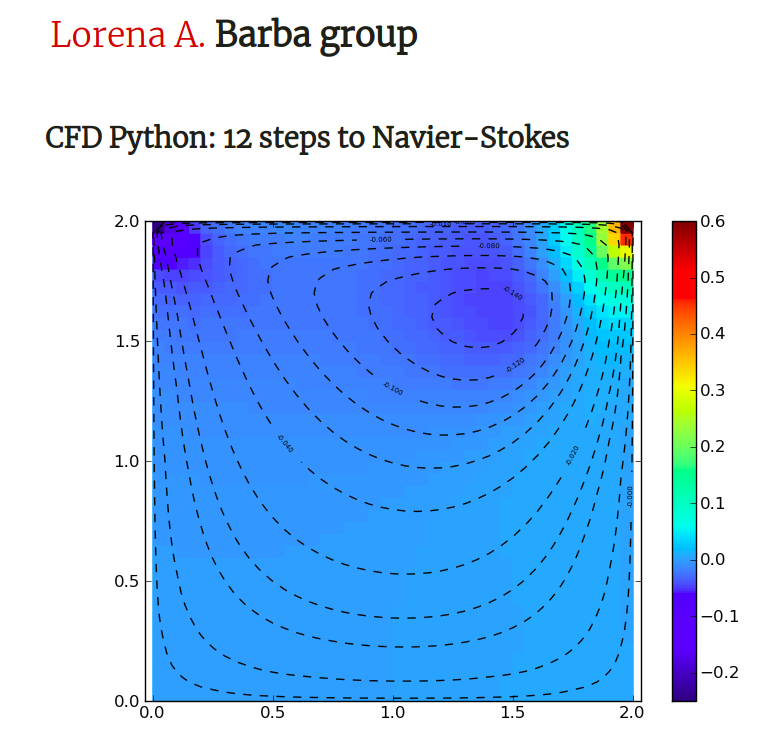
\includegraphics[width=0.80\textwidth]{jupyter_ex_cfd}
			
			\end{figure}
		\end{column}
	\end{columns}	
		
\end{frame}

\begin{frame}[fragile]{Examples}  

"\emph{Introduction to Computational Modelling for the Biosciences}" course in the University of Oslo

\begin{quotation}
One cannot learn programming from slide-based lectures. Much of the learning will have to be done ‘by doing’, in group work. I will use the Jupyter Notebook, the “killer app” in education according to professor Lorena Barba, in a flipped classroom approach where students study notebooks beforehand (each chapter of the course book can be turned into a notebook), formative assessment is used to gauge understanding, and students work with exercises during ‘class’.
	
	\raggedleft	\normalfont --  Lex Nederbragt, the instructor
\end{quotation}

\end{frame}

\begin{frame}[fragile]{Examples}  

	\begin{columns}[t]
		\begin{column}{.3\textwidth}
		Jupyter Notebooks are being used in the "Quantum Mechanics" course and lab of the Pacific University [\href{https://github.com/amcdawes/QMlabs}{Link}]
	
 
		\end{column}
		\begin{column}{.7\textwidth}
			\vspace{-55pt}
			\begin{figure}
			\centering
			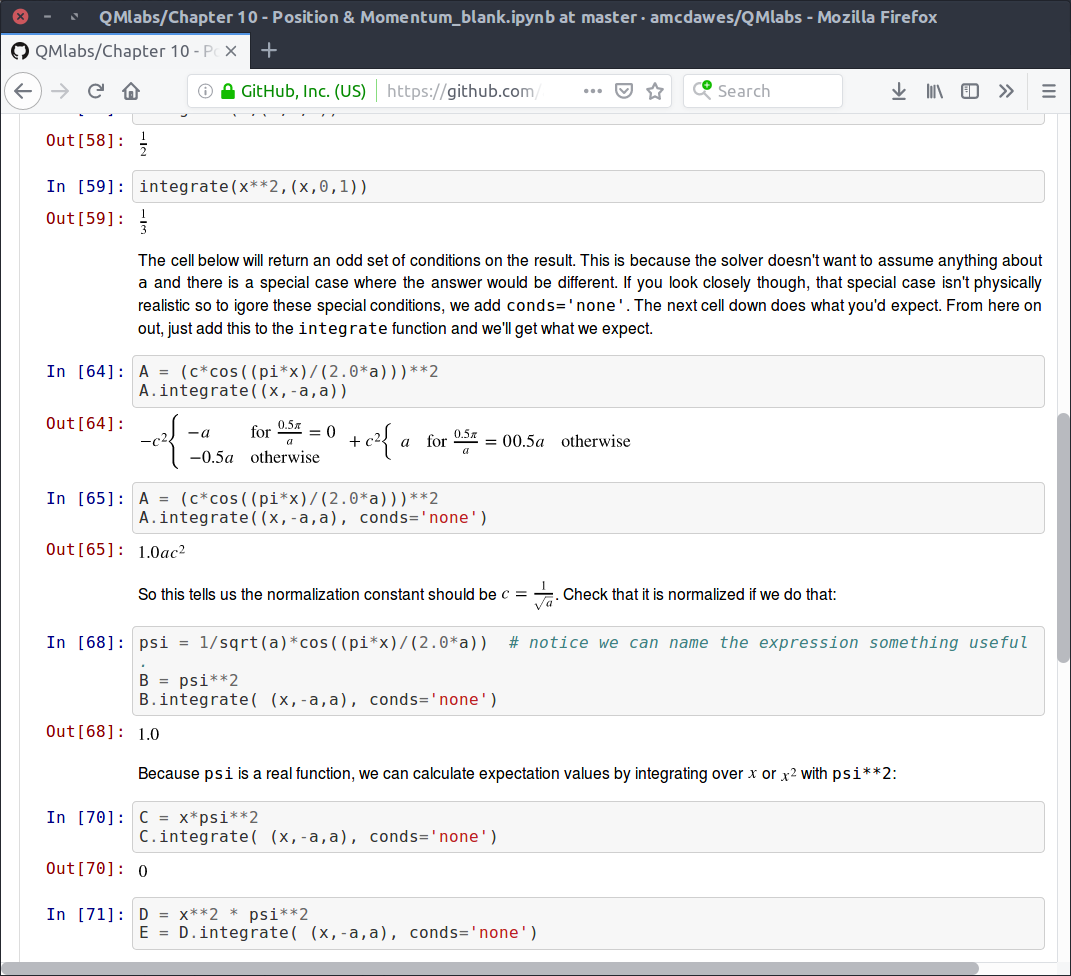
\includegraphics[width=0.80\textwidth]{jupyter_ex_qm}
			
			\end{figure}
		\end{column}
	\end{columns}	
		
\end{frame}

\begin{frame}[fragile]{Examples}  

	\begin{columns}[t]
		\begin{column}{.3\textwidth}
		Jupyter Notebooks in support of "Chemical Process Control" course taught at the University of Notre Dame [\href{http://jckantor.github.io/CBE30338/}{Link}]
	
 
		\end{column}
		\begin{column}{.7\textwidth}
			\vspace{-55pt}
			\begin{figure}
			\centering
			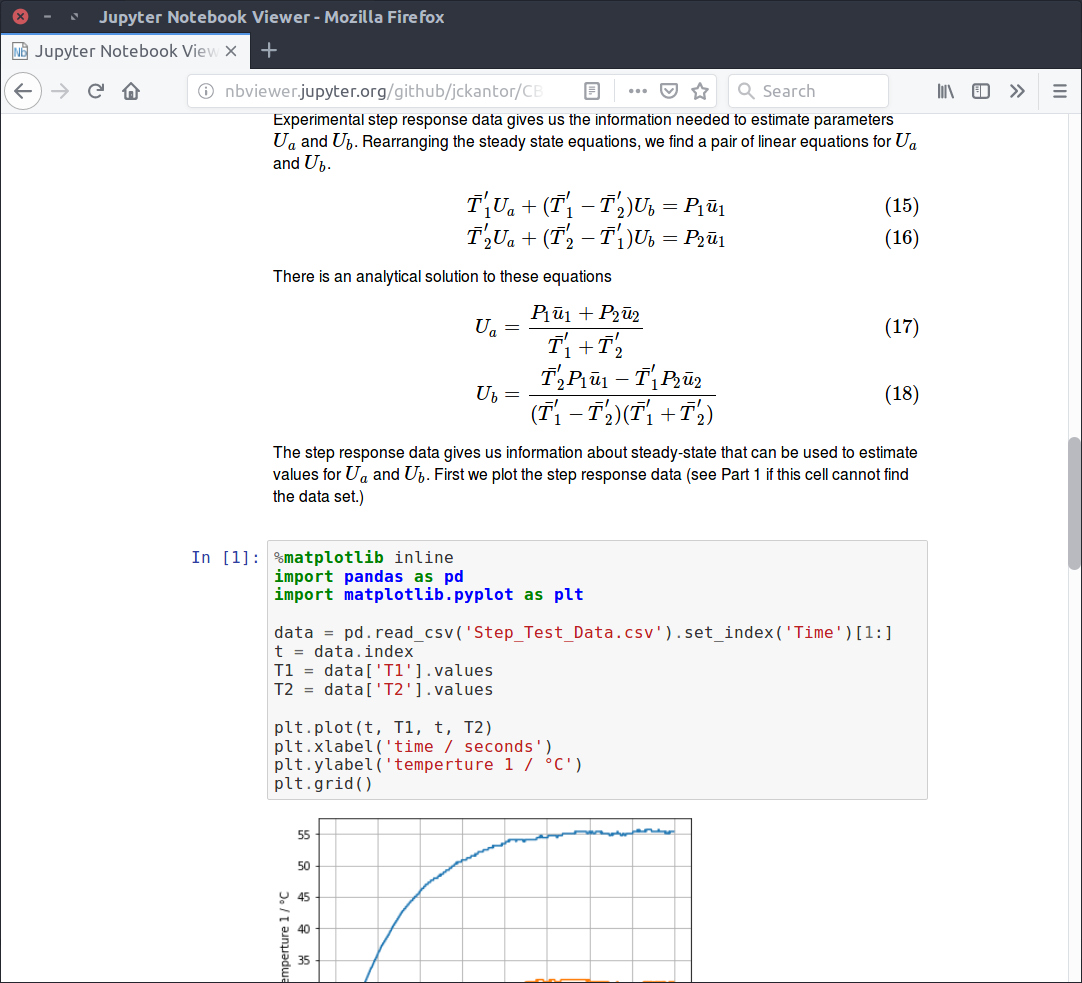
\includegraphics[width=0.80\textwidth]{jupyter_ex_chem}
			
			\end{figure}
		\end{column}
	\end{columns}	
		
\end{frame}

\begin{frame}[fragile]{Examples}  

	\begin{columns}[t]
		\begin{column}{.3\textwidth}
		Sample notebook to animate the $\psi$ wave function [\href{http://nbviewer.jupyter.org/github/atitus/presentations/blob/master/brynmawr-05-19-17/qm-psi-infinite-sq-well.ipynb}{Link}]
	
 
		\end{column}
		\begin{column}{.7\textwidth}
			\vspace{-55pt}
			\begin{figure}
			\centering
			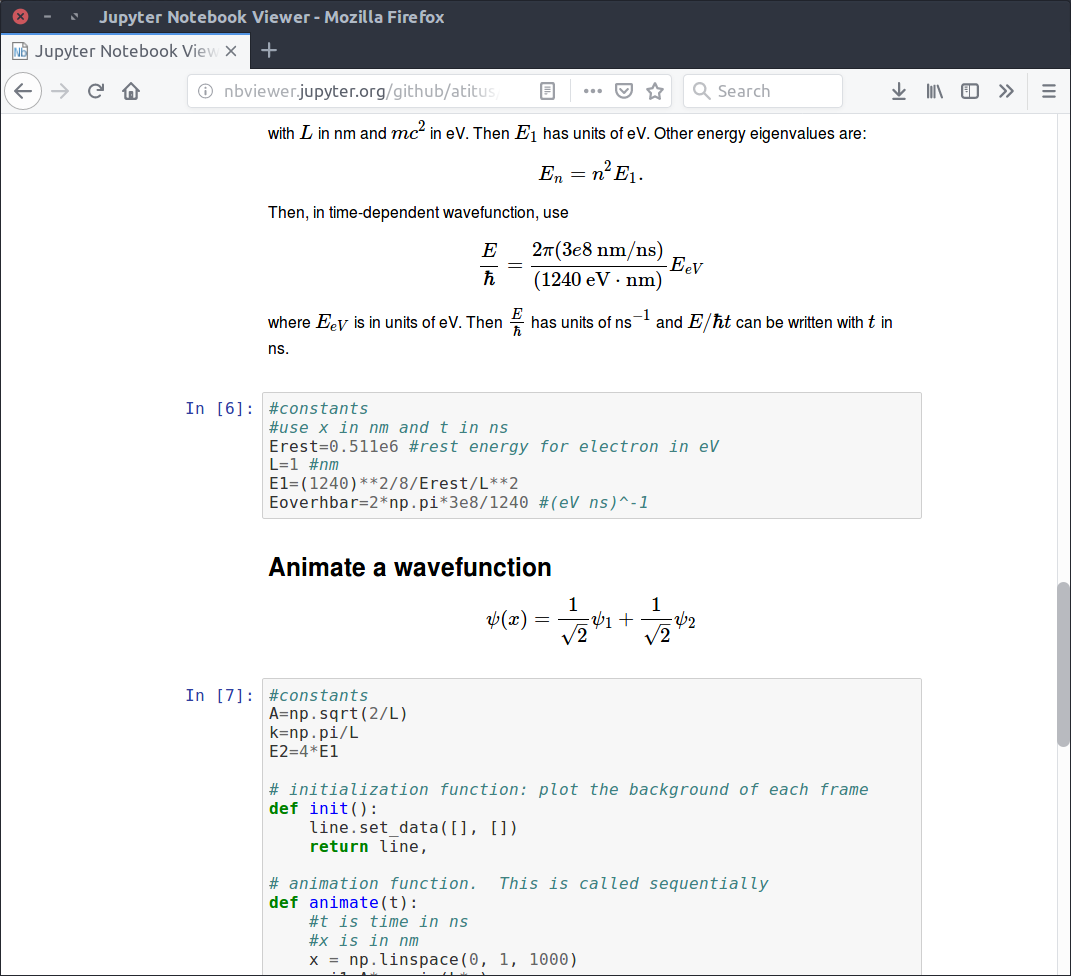
\includegraphics[width=0.80\textwidth]{jupyter_ex_wave}
			
			\end{figure}
		\end{column}
	\end{columns}	
		
\end{frame}

\begin{frame}[fragile]{Examples}  

	\begin{columns}[t]
		\begin{column}{.3\textwidth}
		It has become popular that scientists share the source code of their publications and its corresponding explanations in the notebook format [\href{http://nbviewer.jupyter.org/github/yoavram/ruggedsim/blob/master/manuscript/supplementry.ipynb}{Link}]
	
 
		\end{column}
		\begin{column}{.7\textwidth}
			\vspace{-55pt}
			\begin{figure}
			\centering
			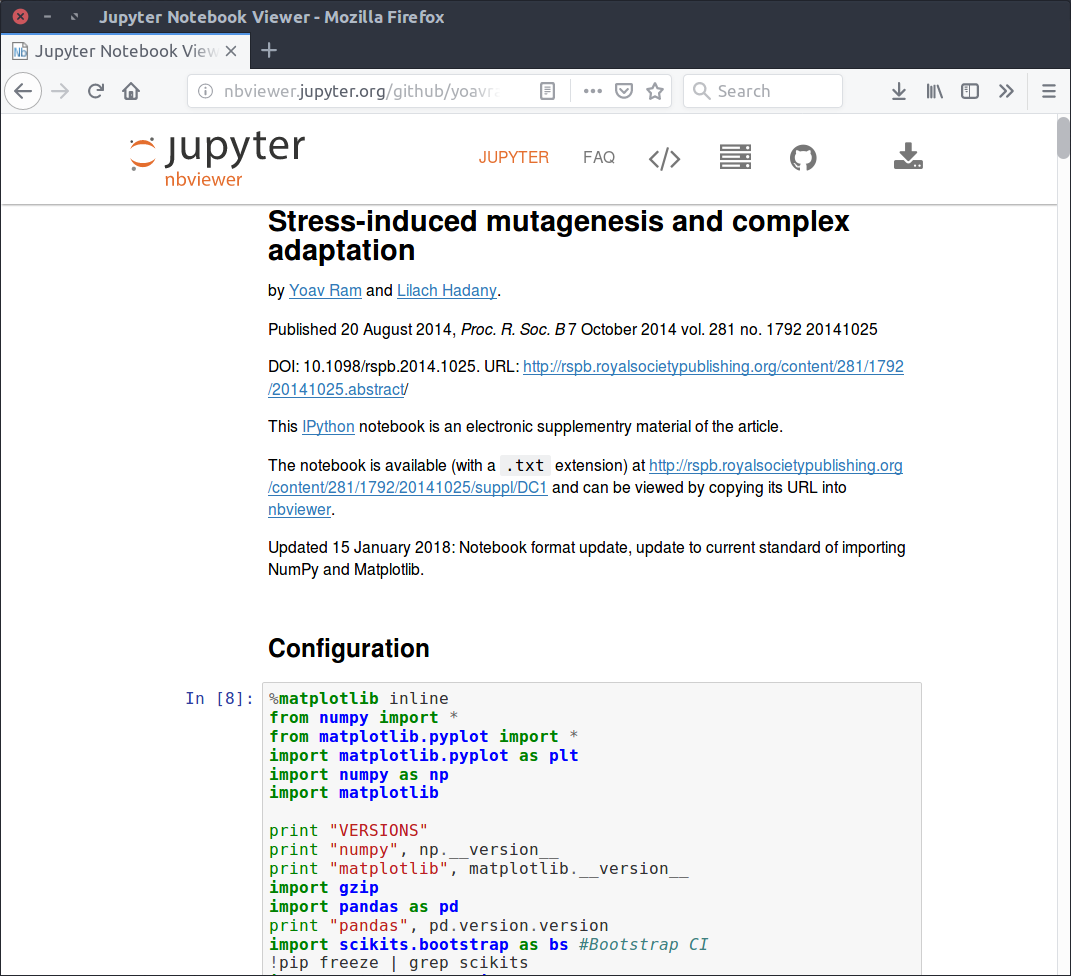
\includegraphics[width=0.80\textwidth]{jupyter_ex_art}
			
			\end{figure}
		\end{column}
	\end{columns}	
		
\end{frame}

\begin{frame}[fragile]{Examples}  

	\begin{columns}[t]
		\begin{column}{.3\textwidth}
		An article to explain the details of a complex topic in Biology step by step using the Jupyter Notebook [\href{http://nbviewer.jupyter.org/github/maayanlab/Zika-RNAseq-Pipeline/blob/master/Zika.ipynb}{Link}]
	
 
		\end{column}
		\begin{column}{.7\textwidth}
			\vspace{-55pt}
			\begin{figure}
			\centering
			
\includegraphics[width=0.80\textwidth]{jupyter_ex_rna}
			
			\end{figure}
		\end{column}
	\end{columns}	
		
\end{frame}

\begin{frame}[fragile]{Examples}  

	\begin{columns}[t]
		\begin{column}{.3\textwidth}
		A sample notebook to demonstrate how to solve the diffusion equation using Finite Different Method in Python [\href{http://nbviewer.jupyter.org/github/waltherg/notebooks/blob/master/2013-12-03-Crank_Nicolson.ipynb}{Link}]
	
 
		\end{column}
		\begin{column}{.7\textwidth}
			\vspace{-55pt}
			\begin{figure}
			\centering
			\includegraphics[width=0.80\textwidth]{jupyter_ex_fdm}
			
			\end{figure}
		\end{column}
	\end{columns}	
		
\end{frame}

\begin{frame}[fragile]{Examples}  

	\begin{columns}[t]
		\begin{column}{.3\textwidth}
		Teaching Physics with Computation
using Jupyter Notebook and VPython at the High Point University [\href{http://nbviewer.jupyter.org/github/atitus/presentations/blob/master/brynmawr-05-19-17/brynmawr-05-19-17.ipynb}{Link}]
	
 
		\end{column}
		\begin{column}{.7\textwidth}
			\vspace{-55pt}
			\begin{figure}
			\centering
			\includegraphics[width=0.80\textwidth]{jupyter_ex_phys}
			
			\end{figure}
		\end{column}
	\end{columns}	
		
\end{frame}

\begin{frame}[fragile]{Examples}  

	\begin{columns}[t]
		\begin{column}{.5\textwidth}
		Textbook Companion open-source project [\href{https://tbc-python.fossee.in/completed-books/}{Link}] aims to create a repository of solved examples of standard engineering textbooks in Jupyter Notebook format, coded in Python.
	
 
		\end{column}
		\begin{column}{.5\textwidth}
			\vspace{-55pt}
			\begin{figure}
			\centering
			\includegraphics[width=0.70\textwidth]{jupyter_ex_book}
			
			\end{figure}
		\end{column}
	\end{columns}	
		
\end{frame}



\begin{frame}[fragile]{Language Support}  
			
Jupyter is not limited to Python and includes a variety of kernels for:
\begin{itemize}
\item
MATLAB
\item
R
\item
C++
\item
Fortran
\item
Java
\item
C\#
\item
Scala
\item
Mathematica
\item
...
\end{itemize}


\end{frame}


\begin{frame}[fragile]{Other Tools and Considerations}  
			
\begin{itemize}
\item
nbgrader
\item
OkPy.org
\item
nbconverter
\item
Hosted Notebooks
\begin{itemize}
\item
JupyterHub (even on a local sever)
\item
Microsoft Azure Notebooks
\item
Anaconda Cloud
\item
...
\end{itemize}
\end{itemize}


\end{frame}


\begin{frame}[fragile]{Time for a Demo!}  
			
			\begin{center}
			Let's create a simple notebook.
			\end{center}

			\begin{figure}
			\centering
			\includegraphics[width=0.6\textwidth]{jupyter_demo}
			
			\end{figure}
\end{frame}


\begin{frame}[fragile]{Wrap It Up}  
			
\begin{itemize}
\item
We can use Jupyter to teach the mathematical modeling of bioreactors step by step, which helps students understand the fundamental concepts of
\begin{itemize}
\item
Mass Transfer
\item
Convection (Advection)
\item
Fluid Flow
\item
Practical Numerical Simulation
\item
\textbf{Real World TE Modeling}
\end{itemize}
in bioreactors and Tissue Engineering.
\item
Jupyter could also be  considered as an effective platform for the assignments of this course and similar courses with a bunch of mathematical and computational operations.
\end{itemize}

\end{frame}

\begin{frame}[plain]{References}  

\footnotesize			
\begin{itemize}
\item
I. Martin et al., The role of bioreactors in tissue
engineering, TRENDS in Biotechnology, 22(2), 2004
\item
J. Hansmann et al., Bioreactors in tissue engineering –
principles, applications and commercial constraints, Biotechnology Journal, 8, 2013
\item
K.J. Blose et al., Bioreactors for Tissue Engineering
Purposes, in book: Regenerative Medicine Applications in Organ Transplantation, 2014
\item
S. J. Hollister, Engineering Scaffold Mechanical and Mass Transport Properties, in book: Comprehensive Biomaterials, 2011
\item
J. Rosser et al., Bioreactor processes for maturation of 3D bioprinted tissue, in book: 3D Bioprinting for Reconstructive Surgery, Techniques and Applications, 2018
\item
E. J. Levorson et al., Scaffolds: Flow Perfusion Bioreactor Design, in book: Comprehensive Biomaterials, 2011
\item
C. Julien et al., Bioreactor Monitoring, Modeling, and Simulation, BioProcess International, 2007
\item
X. Yan et al., Modeling of the Flow within Scaffolds in Perfusion Bioreactors, American Journal of Biomedical Engineering, 1(2), 2011
\item
F. Coletti et al., Mathematical Modeling of Three-Dimensional Cell Cultures in Perfusion Bioreactors, Industrial \& Engineering Chemistry Research, 45, 2006
\end{itemize}

\end{frame}

\begin{frame}[c,plain,noframenumbering]
\begin{tikzpicture}[remember picture,overlay]
\fill[fill=kul-blue]
    (current page.south east)  rectangle  ([shift={(0,-0.1\paperheight)}]current page.north west)   ;
\end{tikzpicture}

\centering
\textcolor{white}{\huge Thank You}
\end{frame}

\end{document}